\documentclass[11pt,a4paper]{article}
\usepackage{fontspec}
\setmainfont[Path=fonts/,FontIndex=7,BoldFont=AvenirNext.ttc,BoldFeatures={FontIndex=2},ItalicFont=AvenirNext.ttc,ItalicFeatures={FontIndex=4},BoldItalicFont=AvenirNext.ttc,BoldItalicFeatures={FontIndex=3}]{AvenirNext.ttc}
\setsansfont[Path=fonts/,FontIndex=7,BoldFont=AvenirNext.ttc,BoldFeatures={FontIndex=2},ItalicFont=AvenirNext.ttc,ItalicFeatures={FontIndex=4},BoldItalicFont=AvenirNext.ttc,BoldItalicFeatures={FontIndex=3}]{AvenirNext.ttc}
\newfontfamily\heavy[Path=fonts/,FontIndex=2]{AvenirNext.ttc}
\setmonofont[Path=fonts/,BoldFont=JetBrainsMono-Bold.ttf,ItalicFont=JetBrainsMono-Italic.ttf,Contextuals=NoAlternate,Ligatures=NoCommon]{JetBrainsMono-Regular.ttf}
\usepackage{xcolor,graphicx,tikz,booktabs,tabularx,listings,amsmath}
\usetikzlibrary{arrows.meta,positioning}
\definecolor{paper}{HTML}{FFFFFF}
\definecolor{ink}{HTML}{252525}
\definecolor{teal}{HTML}{252525}
\definecolor{orange}{HTML}{777777}
\definecolor{wash}{HTML}{EAEAEA}
\definecolor{quiet}{HTML}{666666}
\definecolor{lightink}{HTML}{D0D0D0}
\definecolor{codepaper}{HTML}{F6F6F4}
\lstset{language=Python,basicstyle=\ttfamily\fontsize{9.5}{13}\selectfont\color{ink},keywordstyle=\bfseries\color{ink},commentstyle=\itshape\color{quiet},stringstyle=\color{ink},showstringspaces=false,columns=fullflexible,keepspaces=true,breaklines=true,breakatwhitespace=true,numbers=none,upquote=true,aboveskip=8pt,belowskip=6pt}
\hyphenpenalty=4000
\emergencystretch=3em
% The same two-line navigation and fine rule as the reference, without a candy motif.
\newcommand{\guideheader}[2]{\begin{tikzpicture}[remember picture,overlay]
\node[anchor=north west,inner sep=0,text width=176mm] at ([xshift=16mm,yshift=-7mm]current page.north west) {\fontsize{8.5}{10}\selectfont\color{quiet}#1};
\node[anchor=north west,inner sep=0,text width=176mm] at ([xshift=16mm,yshift=-11.5mm]current page.north west) {\heavy\fontsize{10}{12}\selectfont\color{ink}#2};
\draw[lightink,line width=.4pt] ([xshift=16mm,yshift=-17mm]current page.north west)--([xshift=192mm,yshift=-17mm]current page.north west);
\end{tikzpicture}}

\usepackage[a4paper,left=16mm,right=18mm,top=24mm,bottom=19mm,headheight=14pt]{geometry}
\usepackage{fancyhdr,enumitem,hyperref}
\hypersetup{colorlinks=true,linkcolor=teal,urlcolor=teal}
\setlength{\parindent}{0pt}
\setlength{\parskip}{7pt}
\setlist{nosep,leftmargin=1.4em}
\usepackage{needspace,colortbl}
\lstdefinestyle{numbered}{numbers=left,numberstyle=\ttfamily\fontsize{7.5}{13}\selectfont\color{lightink},numbersep=10pt,xleftmargin=24pt}
\pagestyle{fancy}\fancyhf{}
\fancyhead[C]{\guideheader{\lessonheading}{\nouppercase{\leftmark}}}
\fancyfoot[L]{\fontsize{8}{10}\selectfont\color{quiet}Teacher Class Notes\ifnum\lessonnumber>0\relax\quad /\quad Lesson \lessonnumber\fi}
\fancyfoot[R]{\fontsize{9}{11}\selectfont\color{quiet}\thepage}
\renewcommand{\headrulewidth}{0pt}
\newcommand{\topic}[2]{\clearpage\markboth{#2}{}{\color{quiet}\fontsize{9}{12}\selectfont\textbf{#1}}\par{\heavy\fontsize{19}{23}\selectfont\raggedright #2\par}\vspace{5pt}}
\newcommand{\topicflow}[2]{\par\Needspace{20\baselineskip}\bigskip\markboth{#2}{}{\color{quiet}\fontsize{9}{12}\selectfont\textbf{#1}}\par{\heavy\fontsize{19}{23}\selectfont\raggedright #2\par}\vspace{5pt}}
\newcommand{\labeltext}[1]{{\color{teal}\textbf{#1}}\par}

\newcommand{\lessonnumber}{0}\newcommand{\lessonheading}{Teacher Class Notes}\hypersetup{pdftitle={Dynamic Programming: From Recursion to Efficient Solutions - Teacher Class Notes},pdfauthor={fifteen02},bookmarksopen=true}
\fancyfoot[R]{\heavy\fontsize{10}{12}\selectfont\color{ink}\thepage}
\widowpenalty=10000\clubpenalty=10000\displaywidowpenalty=10000
\begin{document}\color{ink}\fontsize{10.5}{13}\selectfont
\thispagestyle{empty}\null
\begin{tikzpicture}[remember picture,overlay]
\node[anchor=north west,inner sep=0,text width=174mm] at ([xshift=18mm,yshift=-24mm]current page.north west) {\heavy\fontsize{43}{47}\selectfont\raggedright Dynamic\\Programming};
\node[anchor=north west,inner sep=0,text width=174mm] at ([xshift=18mm,yshift=-68mm]current page.north west) {\fontsize{19}{25}\selectfont\raggedright From Recursion to Efficient Solutions};
\node[anchor=north west,inner sep=0,text width=174mm] at ([xshift=18mm,yshift=-94mm]current page.north west) {\heavy\fontsize{15}{19}\selectfont Class Notes\quad {\normalfont\color{quiet}Lessons 1–5}};
\node[anchor=north west,inner sep=0,text width=174mm] at ([xshift=18mm,yshift=-107mm]current page.north west) {\fontsize{12}{16}\selectfont\raggedright Plan the session, ask the questions,\\and work through the answers together.};
\node[anchor=center,inner sep=0] at ([xshift=105mm,yshift=-166mm]current page.north west) {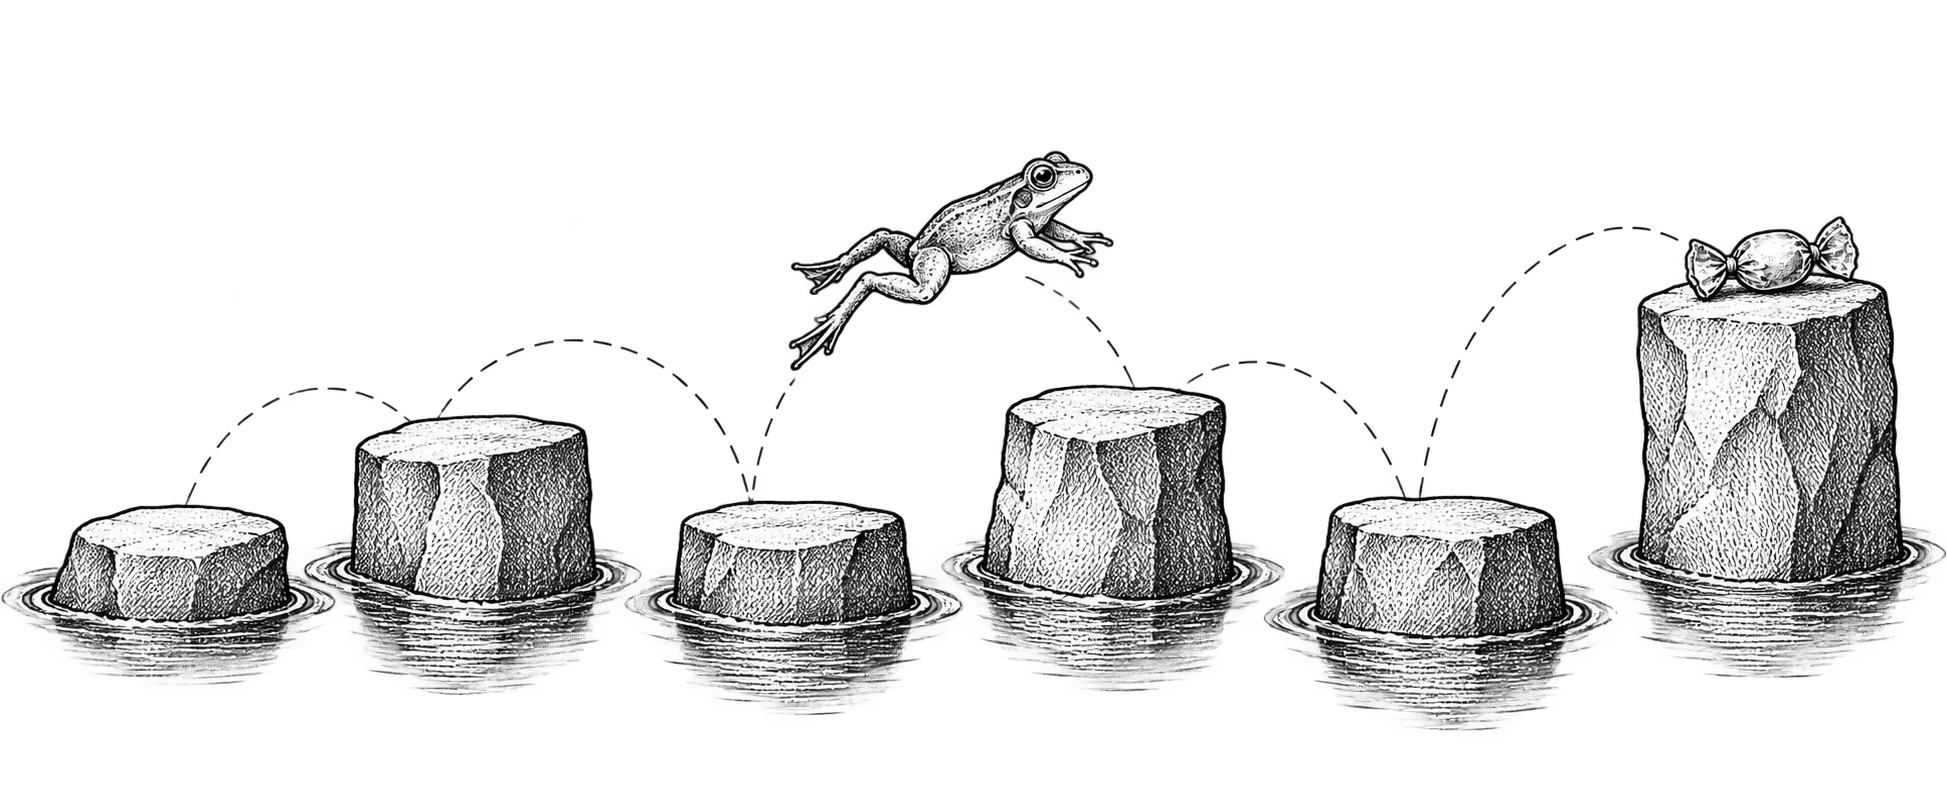
\includegraphics[width=174mm,height=88mm,keepaspectratio]{assets/cover.png}};
\node[anchor=north west,inner sep=0,text width=174mm] at ([xshift=18mm,yshift=-226mm]current page.north west) {\fontsize{12}{16}\selectfont Staircase and Frog · Dice and Grid Paths\\Tower and Array Description · Fruit Feast\\Hoof, Paper, Scissors};
\node[anchor=west,inner sep=0] at ([xshift=18mm,yshift=-269mm]current page.north west) {
\includegraphics[width=43mm]{assets/logo.png}};
\node[anchor=east,inner sep=0] at ([xshift=192mm,yshift=-269mm]current page.north west) {
\includegraphics[width=62mm]{assets/julians-pathfinder-monochrome.pdf}};
\end{tikzpicture}\clearpage
\markboth{Contents}{}\pdfbookmark[0]{Contents}{contents}\noindent\makebox[\linewidth][l]{\begin{minipage}{176mm}{\heavy\fontsize{28}{33}\selectfont Contents\par}\vspace{5mm}
\begin{minipage}{140mm}\raggedright Keep this book open during class. Each lesson contains its timetable, questions, hints, worked answers, completed traces and full code. Give students time to attempt each question before revealing its answer.\end{minipage}\par\vspace{7mm}
\noindent\begin{minipage}[t][29mm][t]{176mm}\vspace{0pt}{\color{lightink}\hrule height .35pt}\vspace{5mm}\begin{minipage}[t]{18mm}\vspace{0pt}{\heavy\fontsize{26}{29}\selectfont 1}\end{minipage}\begin{minipage}[t]{140mm}\vspace{0pt}{\heavy\fontsize{14}{18}\selectfont\hyperref[lesson-1]{Staircase and Frog}\par}\vspace{2mm}{\color{quiet}Remember the answer.}\end{minipage}\begin{minipage}[t]{18mm}\vspace{0pt}\raggedleft{\heavy\fontsize{14}{18}\selectfont\pageref{lesson-1}}\end{minipage}\end{minipage}\par
\noindent\begin{minipage}[t][29mm][t]{176mm}\vspace{0pt}{\color{lightink}\hrule height .35pt}\vspace{5mm}\begin{minipage}[t]{18mm}\vspace{0pt}{\heavy\fontsize{26}{29}\selectfont 2}\end{minipage}\begin{minipage}[t]{140mm}\vspace{0pt}{\heavy\fontsize{14}{18}\selectfont\hyperref[lesson-2]{Dice Combinations and Grid Paths}\par}\vspace{2mm}{\color{quiet}Count the ways to arrive.}\end{minipage}\begin{minipage}[t]{18mm}\vspace{0pt}\raggedleft{\heavy\fontsize{14}{18}\selectfont\pageref{lesson-2}}\end{minipage}\end{minipage}\par
\noindent\begin{minipage}[t][29mm][t]{176mm}\vspace{0pt}{\color{lightink}\hrule height .35pt}\vspace{5mm}\begin{minipage}[t]{18mm}\vspace{0pt}{\heavy\fontsize{26}{29}\selectfont 3}\end{minipage}\begin{minipage}[t]{140mm}\vspace{0pt}{\heavy\fontsize{14}{18}\selectfont\hyperref[lesson-3]{Mortal Kombat Tower and Array Description}\par}\vspace{2mm}{\color{quiet}Remember the missing detail.}\end{minipage}\begin{minipage}[t]{18mm}\vspace{0pt}\raggedleft{\heavy\fontsize{14}{18}\selectfont\pageref{lesson-3}}\end{minipage}\end{minipage}\par
\noindent\begin{minipage}[t][29mm][t]{176mm}\vspace{0pt}{\color{lightink}\hrule height .35pt}\vspace{5mm}\begin{minipage}[t]{18mm}\vspace{0pt}{\heavy\fontsize{26}{29}\selectfont 4}\end{minipage}\begin{minipage}[t]{140mm}\vspace{0pt}{\heavy\fontsize{14}{18}\selectfont\hyperref[lesson-4]{Fruit Feast}\par}\vspace{2mm}{\color{quiet}Track what is possible.}\end{minipage}\begin{minipage}[t]{18mm}\vspace{0pt}\raggedleft{\heavy\fontsize{14}{18}\selectfont\pageref{lesson-4}}\end{minipage}\end{minipage}\par
\noindent\begin{minipage}[t][29mm][t]{176mm}\vspace{0pt}{\color{lightink}\hrule height .35pt}\vspace{5mm}\begin{minipage}[t]{18mm}\vspace{0pt}{\heavy\fontsize{26}{29}\selectfont 5}\end{minipage}\begin{minipage}[t]{140mm}\vspace{0pt}{\heavy\fontsize{14}{18}\selectfont\hyperref[lesson-5]{Hoof, Paper, Scissors}\par}\vspace{2mm}{\color{quiet}Choose when to switch.}\end{minipage}\begin{minipage}[t]{18mm}\vspace{0pt}\raggedleft{\heavy\fontsize{14}{18}\selectfont\pageref{lesson-5}}\end{minipage}\end{minipage}\par
\vspace{5mm}\begin{minipage}{140mm}\raggedright\textbf{Using the two books}\par Teacher Book is for preparation. Teacher Class Notes is for teaching. Question IDs such as L1-04 match the worksheets, slides and notebooks. Each lesson folder holds the classroom materials and practice files.\end{minipage}\end{minipage}}
\clearpage\renewcommand{\lessonnumber}{1}\renewcommand{\lessonheading}{Lesson 1 · Staircase and Frog}\phantomsection\label{lesson-1}\pdfbookmark[-1]{Lesson 1: Staircase and Frog}{lesson-1-bookmark}
\noindent\makebox[\linewidth][l]{\begin{minipage}{176mm}{\heavy\fontsize{23}{28}\selectfont\raggedright Lesson 1\par}\vspace{2mm}{\heavy\fontsize{19}{24}\selectfont\raggedright Staircase and Frog\par}\end{minipage}}\par\vspace{5mm}
\href{https://colab.research.google.com/github/fifteen02/julians-pathfinder/blob/main/Lesson\%201/lesson.ipynb}{\underline{Open this lesson in Google Colab}}\par
\topicflow{BEFORE CLASS}{The lesson route}
\par\noindent\colorbox{wash}{\parbox{\dimexpr\linewidth-2\fboxsep\relax}{\vspace{3pt}{\color{quiet}\heavy\fontsize{8.5}{10}\selectfont MAIN IDEA: SAY THIS AT THE START}\par\smallskip{\heavy\fontsize{15}{18}\selectfont Remember the answer.}\par\smallskip When the same question comes up again, reuse its saved answer instead of working it out again.\par\medskip\textbf{By the end of the lesson you will be able to}\begin{itemize}\item read a function that calls itself and explain how it stops;\item count staircase routes, then save answers that are needed again;\item solve Frog using exhaustive recursion, caching and an iterative table.\end{itemize}\vspace{3pt}}}\par

The target is understanding, not finishing every page. Use the question IDs to move between slides, worksheet and notebook. Questions labelled optional are extensions.

\begingroup\small\setlength{\tabcolsep}{4pt}\renewcommand{\arraystretch}{1.35}\begin{tabularx}{\linewidth}{>{\raggedright\arraybackslash}p{18mm}>{\raggedright\arraybackslash}X>{\raggedright\arraybackslash}p{38mm}}\toprule\textbf{Minutes} & \textbf{Activity} & \textbf{Question IDs}\\\midrule
0-8 & Recursion refresher: trace one call and identify the base case & L1-01 to L1-04\\
8-18 & Board: staircase routes and the last move & L1-05 to L1-06\\
18-30 & Stopping cases and the slow staircase program & L1-07 to L1-08\\
30-42 & Repeated calls, caching and depth & L1-09 to L1-11\\
42-52 & Fill the staircase table in order & L1-12\\
52-60 & Students change the allowed jumps & L1-13\\
60-65 & Break & \\
65-78 & Frog: whole-route costs and a greedy counterexample & L1-14 to L1-15\\
78-93 & Frog: exhaustive recursion, then caching & L1-16 to L1-17\\
93-110 & Frog: build the iterative solution and test it & L1-18 to L1-19\\
110-120 & Compare the two tables; exit question & L1-20\\
\bottomrule\end{tabularx}\endgroup

\labeltext{Pacing and preparation}
Ask students to predict before running code. Allow a quiet individual attempt before asking for a volunteer. If an answer is wrong, trace the first state where it differs. Keep the final ten minutes for explanation and questions. Move an unfinished implementation to the next session rather than shortening the reasoning.

Students need Python functions, lists, loops, indexing, comparisons and basic arithmetic. Introduce new syntax beside the program that uses it. Use small inputs for uncached recursion; the notebook never starts an enormous recursive run. Python stops recursion at about 1,000 nested calls by default, so every recursive version in this lesson, cached or not, is for small inputs and the small and edge test files only. The medium and large files are for the iterative versions.

L1-21 adds route recovery after the cost solution. Allow 15-20 extra minutes or use it as a follow-up; it is outside the two-hour core.

Open lesson.ipynb in Jupyter or upload it to Google Colab, choose a Python 3 runtime, and run the setup cell first. Shift+Enter runs a cell. Restart and run from the top if names or data become stale. The notebook needs only Python standard-library features and no local files.
\topic{KEEP BESIDE YOUR WORK}{The route and the rules}
\textbf{Our route}\par Start with a brief recursion refresher; choose one warm-up exercise if you already know how calls stop. Then count staircase routes by hand. Write a recursive function, see which questions repeat, and save their answers. Then fill the same answers with a loop. Change the allowed jumps before trying Frog, where the answer is a minimum cost instead of a count.\par\medskip
\textbf{Recursion warm-up · L1-01 to L1-04}\par A function may call itself on a smaller input. The base case answers directly, without another call; every other call must move closer to the base case. A call that is waiting for a smaller call stays unfinished until that call returns its value.\par\medskip
\textbf{Staircase rules · L1-05 to L1-13}\par Start at ground level, called step 0. A move climbs exactly 1 or 2 steps. Count ordered lists of moves that land exactly on the target. For example, [1, 2] and [2, 1] are different routes. In L1-13 only, the permitted moves change to 1 or 3.\par\medskip
\textbf{Frog rules · L1-14 to L1-20}\par Number the stones 0, 1, 2 and so on. Start on stone 0 and finish on the last stone. A jump moves forward by one or two stone positions. Its cost is the absolute height difference: a jump from height 50 to height 30 costs 20. Add every jump cost in a route; find the smallest total.\par\medskip
\textbf{Names used in the questions}\par \texttt{ways(n)} is a function returning the number of staircase routes to target step n. \texttt{ways[n]} is a list entry storing that count. Parentheses call a function; square brackets read a stored entry. In Frog, \texttt{heights[i]} is the height at stone position i, while \texttt{best[i]} is the cheapest total cost to reach it.\par\medskip
\textbf{What to complete in class}\par Complete both staircase and Frog: for each, follow the slow recursive solution, save repeated answers, then fill a table with a loop. The recursion warm-up is a short refresher; the remaining warm-up exercises can be used for extra practice. Explain each small example before running a large input.\par\medskip
\topicflow{IN CLASS}{Questions, answers and prompts}
\labeltext{Recursion warm-up (before L1-01; slides 3 to 7)}
Objective: students read and write a function that calls itself, so that the staircase recursion is not their first recursive function. Teach in this order, using the slides: (1) a function may call itself on a smaller input (countdown); (2) the two parts: base case and smaller case; (3) a waiting call stays on the call stack until the smaller call returns; (4) show the incomplete sum\_to(3) table and ask students to predict each returned value; (5) reveal the completed table on the following slide, after their attempt. Do not reveal the countdown output before L1-01. In the notebook, predictions come before the runnable checks and the closed answer panels. Allow eight minutes for this refresher. Use one of L1-01 to L1-04 to check understanding; keep the others as optional practice if students already know recursion. Continue to the staircase by minute 8 so that the full Frog progression fits after the break.

\textbf{Worked example for the board.}
\begin{lstlisting}
def sum_to(n):
    if n == 0:
        return 0
    return n + sum_to(n - 1)
\end{lstlisting}
\begingroup\small\setlength{\tabcolsep}{5pt}\setlength{\arrayrulewidth}{.5pt}\arrayrulecolor{quiet}\renewcommand{\arraystretch}{1}\begin{tabularx}{\linewidth}{|>{\raggedright\arraybackslash}p{19mm}|>{\centering\arraybackslash}X|>{\centering\arraybackslash}X|}\hline
\rowcolor{wash}\rule[-2mm]{0pt}{6.5mm}\textbf{Call} & \textbf{Waits for} & \textbf{Returns}\\\hline
\rule[-2.7mm]{0pt}{8mm}sum\_to(3) & sum\_to(2) & 3 + 3 = 6\\\hline
\rule[-2.7mm]{0pt}{8mm}sum\_to(2) & sum\_to(1) & 2 + 1 = 3\\\hline
\rule[-2.7mm]{0pt}{8mm}sum\_to(1) & sum\_to(0) & 1 + 0 = 1\\\hline
\rule[-2.7mm]{0pt}{8mm}sum\_to(0) & nothing (base case) & 0\\\hline
\end{tabularx}\endgroup\par\medskip
\markboth{Warm-up: functions that call themselves}{}{\color{quiet}\heavy\fontsize{10}{13}\selectfont WARM-UP: FUNCTIONS THAT CALL THEMSELVES}\par\medskip
\noindent\begin{minipage}{\textwidth}
{\color{teal}\textbf{L1-01}}\quad \textbf{A function that calls itself}\par\smallskip
\textbf{Ask.} A function may call itself on a smaller input. countdown(n) below prints n and then calls countdown(n - 1); when n is 0 it prints Go! and makes no further call. In the table, write every call that countdown(3) makes, in order, what that call prints and which call it makes next.\par\smallskip
{\small\textbf{Code printed with the question.}}\par\smallskip\noindent\colorbox{codepaper}{\parbox{\dimexpr\linewidth-2\fboxsep\relax}{\small\ttfamily\raggedright def countdown(n):\\\hspace*{2.4em}if n == 0:\\\hspace*{4.8em}print('Go!')\\\hspace*{4.8em}return\\\hspace*{2.4em}print(n)\\\hspace*{2.4em}countdown(n - 1)}}\par
\smallskip\textbf{Answer.} Read the completed table from top to bottom. Each call prints before making the next call; the base case makes no further call.\par\smallskip
\textbf{Prompt if stuck.} Which call prints Go!, and does it call anything?\par\smallskip
\textbf{Watch for.} Calling countdown(n - 1) does not jump back to the top of the same call; it starts a new call with its own n.
\end{minipage}\par\medskip{\color{lightink}\hrule height .4pt}\medskip

\noindent\begin{minipage}{\textwidth}
{\color{teal}\textbf{L1-02}}\quad \textbf{Wait for the smaller answer}\par\smallskip
\textbf{Ask.} sum\_squares(n) returns 0 when n is 0; otherwise it returns n * n + sum\_squares(n - 1). A call cannot finish until the call it waits for has returned. Fill the table for sum\_squares(4), starting from the bottom row and working up. Write the addition for each returned value.\par\smallskip
{\small\textbf{Code printed with the question.}}\par\smallskip\noindent\colorbox{codepaper}{\parbox{\dimexpr\linewidth-2\fboxsep\relax}{\small\ttfamily\raggedright def sum\_squares(n):\\\hspace*{2.4em}if n == 0:\\\hspace*{4.8em}return 0\\\hspace*{2.4em}return n * n + sum\_squares(n - 1)}}\par
\smallskip\textbf{Answer.} Fill the returned values from the bottom row upward. Each call adds its own square to the value returned by the next row.\par\smallskip
\textbf{Prompt if stuck.} Which row can you fill without knowing any other row?\par\smallskip
\textbf{Watch for.} Writing 4 * 4 = 16 as the returned value forgets the waiting part: each call adds its own square to the value returned by the smaller call.
\end{minipage}\par\medskip{\color{lightink}\hrule height .4pt}\medskip

\noindent\begin{minipage}{\textwidth}
{\color{teal}\textbf{L1-03}}\quad \textbf{Find the missing base case}\par\smallskip
\textbf{Ask.} power2(n) below should return 2 to the power n: 2 multiplied by itself n times, so power2(3) should be 8. What happens when you call power2(3)? Which value of n can you answer directly, without a smaller call? Add that base case and check that power2(3) now returns 8.\par\smallskip
{\small\textbf{Code printed with the question.}}\par\smallskip\noindent\colorbox{codepaper}{\parbox{\dimexpr\linewidth-2\fboxsep\relax}{\small\ttfamily\raggedright def power2(n):\\\hspace*{2.4em}return 2 * power2(n - 1)}}\par
\smallskip\par\smallskip{\small\textbf{Students start with:}}\par\smallskip\noindent\colorbox{codepaper}{\parbox{\dimexpr\linewidth-2\fboxsep\relax}{\small\ttfamily\raggedright def power2(n):\\\hspace*{2.4em}return None  \# Replace with your answer.}}\par
{\small\textbf{What each function returns.}\par power2(n): the integer 2 raised to the power n.\par }
{\small\textbf{Hints to give, one at a time.}}\begin{itemize}\item Trace the inputs until they pass 0. Where should the chain stop?\item Check your repaired function on the stopping input before trying 3.\end{itemize}
\textbf{Answer.} The incomplete version continues past input 0 until Python raises RecursionError. Check n == 0 before the smaller call and return 1 there. The completed trace below uses that stopping case.\par\smallskip
\textbf{Prompt if stuck.} Follow the arguments 3, 2, 1, 0, -1. Where should the calls stop, and what is 2 to the power 0?\par\smallskip
\textbf{Watch for.} A base case that is placed after the recursive call is never reached.\par\smallskip Full code: \texttt{power2} (page~\pageref{L1-code-power2}).
\end{minipage}\par\medskip{\color{lightink}\hrule height .4pt}\medskip

\noindent\begin{minipage}{\textwidth}
{\color{teal}\textbf{L1-04}}\quad \textbf{Write a recursive function}\par\smallskip
\textbf{Ask.} factorial(n) is the product 1 × 2 × ... × n, and factorial(0) is 1. Write factorial(n) recursively: first the base case, then one smaller call. Predict factorial(4) before running it. The staircase that follows uses the same pattern, with two smaller calls instead of one.\par\smallskip
\par\smallskip{\small\textbf{Students start with:}}\par\smallskip\noindent\colorbox{codepaper}{\parbox{\dimexpr\linewidth-2\fboxsep\relax}{\small\ttfamily\raggedright def factorial(n):\\\hspace*{2.4em}return None  \# Replace with your answer.}}\par
{\small\textbf{What each function returns.}\par factorial(n): the product of integers 1 through n; for n = 0, return 1.\par }
{\small\textbf{Hints to give, one at a time.}}\begin{itemize}\item What is the smallest n you can answer directly?\item If you already knew factorial(n - 1), what single step would give factorial(n)?\end{itemize}
\textbf{Answer.} Return 1 at input 0. For a positive input, multiply that input by the result of the call with input one smaller. The table shows the returned values.\par\smallskip
\textbf{Prompt if stuck.} What is factorial(0)? How is factorial(4) related to factorial(3)?\par\smallskip
\textbf{Watch for.} Returning n * factorial(n) never reaches the base case; the argument must get smaller.\par\smallskip Full code: \texttt{factorial} (page~\pageref{L1-code-factorial}).
\end{minipage}\par\medskip{\color{lightink}\hrule height .4pt}\medskip

\Needspace{14\baselineskip}\markboth{Staircase: count, remember, then loop}{}{\color{quiet}\heavy\fontsize{10}{13}\selectfont STAIRCASE: COUNT, REMEMBER, THEN LOOP}\par\medskip
\noindent\begin{minipage}{\textwidth}
{\color{teal}\textbf{L1-05}}\quad \textbf{Five steps, many routes}\par\smallskip
\textbf{Ask.} Start on the ground, called step 0. Each move climbs exactly 1 or 2 steps. Count routes that land exactly on each target from step 1 to step 5. List the routes to step 5 as move lists, such as [1, 2, 2]. Does changing the order make a different route?\par\smallskip
\textbf{Answer.} Steps 1 through 5 have 1, 2, 3, 5 and 8 routes. The routes to step 5 are 11111, 1112, 1121, 1211, 2111, 122, 212, 221. Each digit is one move. Order matters: 122 and 212 visit different steps.\par\smallskip
\textbf{Prompt if stuck.} First list routes to steps 1, 2 and 3. Extend only routes that land exactly on the target.\par\smallskip
\textbf{Watch for.} Treating 122 and 212 as the same combination loses valid ordered routes.
\end{minipage}\par\medskip{\color{lightink}\hrule height .4pt}\medskip

\noindent\begin{minipage}{\textwidth}
{\color{teal}\textbf{L1-06}}\quad \textbf{The last move explains the sum}\par\smallskip
\textbf{Ask.} The next move must land on step 5. Where can that move start? Use your L1-05 counts for step 4 and step 3. How can these two counts give the answer for step 5?\par\smallskip
\textbf{Answer.} The last move starts at step 4 with a jump of 1, or at step 3 with a jump of 2. Extend each earlier route once. The groups cannot overlap because their last moves differ: 5 + 3 = 8.\par\smallskip
\textbf{Prompt if stuck.} Remove the final move from any completed route. What step remains?\par\smallskip
\textbf{Watch for.} Adding step numbers 4 + 3 is different from adding their route counts 5 + 3.
\end{minipage}\par\medskip{\color{lightink}\hrule height .4pt}\medskip

\noindent\begin{minipage}{\textwidth}
{\color{teal}\textbf{L1-07}}\quad \textbf{Where recursion stops}\par\smallskip
\textbf{Ask.} Let ways(n) return the number of routes from the ground to target step n, using jumps of 1 or 2. What should ways(0) and ways(-1) return? Use these answers to work out ways(1).\par\smallskip
\textbf{Answer.} ways(0) = 1: the empty list is one way to climb zero steps. ways(-1) = 0: positive jumps cannot finish below the ground. Therefore ways(1) = ways(0) + ways(-1) = 1.\par\smallskip
\textbf{Prompt if stuck.} How many lists of positive moves have sum zero?\par\smallskip
\textbf{Watch for.} Returning zero for ways(0) makes every later count zero.
\end{minipage}\par\medskip{\color{lightink}\hrule height .4pt}\medskip

\noindent\begin{minipage}{\textwidth}
{\color{teal}\textbf{L1-08}}\quad \textbf{The slow recursive program}\par\smallskip
\textbf{Ask.} Write stairs\_slow(n), the number of staircase routes to step n with jumps of 1 or 2. Start with the stopping cases, then ask about the two possible starting steps of the final jump. Draw every call made for stairs\_slow(3) and write the returned count beside it.\par\smallskip
\par\smallskip{\small\textbf{Students start with:}}\par\smallskip\noindent\colorbox{codepaper}{\parbox{\dimexpr\linewidth-2\fboxsep\relax}{\small\ttfamily\raggedright def stairs\_slow(n):\\\hspace*{2.4em}return None  \# Replace with your answer.}}\par
{\small\textbf{What each function returns.}\par stairs\_slow(n): the number of ordered routes to step n using jumps of 1 or 2.\par }
{\small\textbf{Hints to give, one at a time.}}\begin{itemize}\item Which targets can you answer without a smaller call? Think about 0 and about negative targets.\item The last move is 1 or 2 steps. Which smaller targets do those leave?\end{itemize}
\textbf{Answer.} stairs\_slow(3) returns 3. It calls stairs\_slow(2) and stairs\_slow(1); stairs\_slow(2) calls stairs\_slow(1) and stairs\_slow(0). Each stairs\_slow(1) calls stairs\_slow(0) and stairs\_slow(-1). Return 1 at target 0 and 0 at target -1. Then stairs\_slow(1) returns 1, stairs\_slow(2) returns 2, and stairs\_slow(3) returns 2 + 1 = 3.\par\smallskip
\textbf{Prompt if stuck.} Put the base cases before the recursive return.\par\smallskip
\textbf{Watch for.} A recursive call returns a number. It does not automatically store that number for another call.\par\smallskip Full code: \texttt{stairs\_slow} (page~\pageref{L1-code-stairs_slow}).
\end{minipage}\par\medskip{\color{lightink}\hrule height .4pt}\medskip

\noindent\begin{minipage}{\textwidth}
{\color{teal}\textbf{L1-09}}\quad \textbf{Repeated questions in the call tree}\par\smallskip
\textbf{Ask.} The diagram shows the first three levels of calls made while counting routes to step 5. Circle calls with the same input. What work does the second call to ways(3) repeat?\par\smallskip
\textbf{Answer.} The displayed levels contain two calls to ways(3) and two to ways(2). Each call to ways(3) asks for the same route count, but both rebuild its smaller calls. The drawing stops early: each displayed call with a positive input would continue branching until a stopping case.\par\smallskip
\textbf{Prompt if stuck.} Look for identical function names with identical arguments.\par\smallskip
\textbf{Watch for.} The number of calls can grow exponentially even though the depth grows only linearly.
\end{minipage}\par\medskip{\color{lightink}\hrule height .4pt}\medskip

\noindent\begin{minipage}{\textwidth}
{\color{teal}\textbf{L1-10}}\quad \textbf{A cache keeps an answer}\par\smallskip
\textbf{Ask.} A cache is a dictionary that saves an answer under the input that produced it. We have found 5 routes to step 4. Complete cache[?] = ?. What should a later call to ways(4) return, and which work can it skip?\par\smallskip
\textbf{Answer.} Store cache[4] = 5. Key 4 identifies the step. Value 5 is its route count. A later call reads 5 immediately instead of exploring ways(3) and ways(2) again.\par\smallskip
\textbf{Prompt if stuck.} The key describes the question; the stored value answers it.\par\smallskip
\textbf{Watch for.} Recreating the dictionary inside every recursive call prevents sharing.\par\smallskip Full code: \texttt{stairs\_cached} (page~\pageref{L1-code-stairs_cached}).
\end{minipage}\par\medskip{\color{lightink}\hrule height .4pt}\medskip

\noindent\begin{minipage}{\textwidth}
{\color{teal}\textbf{L1-11}}\quad \textbf{Fast work can still mean deep recursion}\par\smallskip
\textbf{Ask.} Caching removes repeated work. Why can a large staircase input still cause RecursionError in Python? What does iteration change?\par\smallskip
\textbf{Answer.} The calls for n, n - 1, n - 2 and so on can remain active together. Caching does not shorten that chain. Python limits nested calls. A loop fills answers without building this recursive call chain.\par\smallskip
\textbf{Prompt if stuck.} Imagine all the calls waiting for the smallest question to return.\par\smallskip
\textbf{Watch for.} Fast enough in operation count does not mean safe in recursion depth.\par\smallskip Full code: \texttt{recursion\_demo} (page~\pageref{L1-code-recursion_demo}).
\end{minipage}\par\medskip{\color{lightink}\hrule height .4pt}\medskip

\noindent\begin{minipage}{\textwidth}
{\color{teal}\textbf{L1-12}}\quad \textbf{Build the table in order}\par\smallskip
\textbf{Ask.} Write stairs\_table(n) using a loop. First fill ways[step], the route count, for steps 0 through 5. Which earlier count is available at step 1? Which two are needed from step 2 onwards? Use that order in your code.\par\smallskip
\par\smallskip{\small\textbf{Students start with:}}\par\smallskip\noindent\colorbox{codepaper}{\parbox{\dimexpr\linewidth-2\fboxsep\relax}{\small\ttfamily\raggedright def stairs\_table(n):\\\hspace*{2.4em}return None  \# Replace with your answer.}}\par
{\small\textbf{What each function returns.}\par stairs\_table(n): the number of ordered routes to step n using jumps of 1 or 2.\par }
{\small\textbf{Hints to give, one at a time.}}\begin{itemize}\item How long must the list be so that ways[n] exists?\item Which entry do you know before the loop starts?\item When you fill ways[step], which entries must already be filled?\end{itemize}
\textbf{Answer.} The counts are [1, 1, 2, 3, 5, 8]. Step 1 reads only ways[0]. Each step s from 2 onwards reads ways[s - 1] and ways[s - 2]. For step 5, those counts are 5 and 3, giving 8. Increasing step order ensures both earlier answers exist.\par\smallskip
\textbf{Prompt if stuck.} Write the positions above the counts, not in the same row.\par\smallskip
\textbf{Watch for.} Forgetting position 0 leads to an off-by-one error in the allocated list.\par\smallskip Full code: \texttt{stairs\_table} (page~\pageref{L1-code-stairs_table}).
\end{minipage}\par\medskip{\color{lightink}\hrule height .4pt}\medskip

\noindent\begin{minipage}{\textwidth}
{\color{teal}\textbf{L1-13}}\quad \textbf{Your turn: jumps of 1 or 3}\par\smallskip
\textbf{Ask.} Write stairs\_13(n) by adapting stairs\_table from L1-12. Allow only jumps of 1 or 3, never 2. First fill the counts for steps 0 through 7, then write and test your code.\par\smallskip
\par\smallskip{\small\textbf{Students start with:}}\par\smallskip\noindent\colorbox{codepaper}{\parbox{\dimexpr\linewidth-2\fboxsep\relax}{\small\ttfamily\raggedright def stairs\_13(n):\\\hspace*{2.4em}return None  \# Replace with your answer.}}\par
{\small\textbf{What each function returns.}\par stairs\_13(n): the number of ordered routes to step n using jumps of 1 or 3.\par }
{\small\textbf{Hints to give, one at a time.}}\begin{itemize}\item Which line of stairs\_table depends on the allowed jumps?\item A jump can only start from a step that exists. What must be true before you read an earlier entry?\end{itemize}
\textbf{Answer.} The counts are [1, 1, 1, 2, 3, 4, 6, 9]. For step 7, the last jump begins at step 6 or step 4, giving 6 + 3 = 9. Use jumps (1, 3) and ignore negative predecessor steps.\par\smallskip
\textbf{Prompt if stuck.} List the allowed final jumps explicitly: (1, 3).\par\smallskip
\textbf{Watch for.} Using range(1, 4) also allows the forbidden jump of 2.\par\smallskip Full code: \texttt{stairs\_13} (page~\pageref{L1-code-stairs_13}).
\end{minipage}\par\medskip{\color{lightink}\hrule height .4pt}\medskip

\Needspace{14\baselineskip}\markboth{Frog: compare complete route costs}{}{\color{quiet}\heavy\fontsize{10}{13}\selectfont FROG: COMPARE COMPLETE ROUTE COSTS}\par\medskip
\noindent\begin{minipage}{\textwidth}
{\color{teal}\textbf{L1-14}}\quad \textbf{Frog: cost belongs to a whole route}\par\smallskip
\textbf{Ask.} Number the stones 0, 1 and 2; their heights are [10, 20, 30]. A frog starts at stone 0 and may jump forward one or two positions. A jump costs the absolute height difference, so a drop of 10 also costs 10. List all routes to stone 2 and add the jump costs for each.\par\smallskip
\textbf{Answer.} The routes are 0, 1, 2 with cost 10 + 10 = 20, and 0, 2 with cost 20. Both are optimal. A cost is never negative: abs(10 - 30) = 20.\par\smallskip
\textbf{Prompt if stuck.} The two permitted next positions are i + 1 and i + 2, if they exist.\par\smallskip
\textbf{Watch for.} Minimising the number of jumps is not the same as minimising height-difference cost.
\end{minipage}\par\medskip{\color{lightink}\hrule height .4pt}\medskip

\noindent\begin{minipage}{\textwidth}
{\color{teal}\textbf{L1-15}}\quad \textbf{A greedy choice can fail}\par\smallskip
\textbf{Ask.} Use heights [20, 50, 30, 40, 10, 10], at stones 0 through 5. At each stone, choose the cheaper of the next two legal jumps; if costs tie, choose the farther stone. Trace this greedy route and its total cost. Can another complete route cost less?\par\smallskip
\textbf{Answer.} Greedy can take stones 0, 2, 3, 5: cost 10 + 10 + 30 = 50. The optimal route 0, 2, 4, 5 costs 10 + 20 + 0 = 30. Paying more at stone 2 saves cost later.\par\smallskip
\textbf{Prompt if stuck.} Compare what happens after choosing stone 3 with what happens after choosing stone 4.\par\smallskip
\textbf{Watch for.} Calling greedy brute force hides the distinction between a wrong shortcut and a correct but slow search.
\end{minipage}\par\medskip{\color{lightink}\hrule height .4pt}\medskip

\noindent\begin{minipage}{\textwidth}
{\color{teal}\textbf{L1-16}}\quad \textbf{Frog: ask about the last jump}\par\smallskip
\textbf{Ask.} Write frog\_slow(heights) with recursive helper cost(i): the cheapest total cost from stone 0 to stone i. Which earlier stones can supply the last jump? Explore both possibilities.\par\smallskip
\par\smallskip{\small\textbf{Students start with:}}\par\smallskip\noindent\colorbox{codepaper}{\parbox{\dimexpr\linewidth-2\fboxsep\relax}{\small\ttfamily\raggedright def frog\_slow(heights):\\\hspace*{2.4em}def cost(i):\\\hspace*{4.8em}return None  \# Your helper goes here.\\\hspace*{2.4em}return cost(len(heights) - 1)}}\par
{\small\textbf{What each function returns.}\par frog\_slow(heights): the cheapest total cost from stone 0 to the last stone.\par cost(i): the cheapest total cost from stone 0 to stone i, including all jumps along the route.\par }
{\small\textbf{Hints to give, one at a time.}}\begin{itemize}\item What is the smallest i you can answer directly?\item Which earlier stones can the last jump into stone i start from?\item What does cost(i) need to know about each of those stones?\end{itemize}
\textbf{Answer.} Try i - 1 and, when it exists, i - 2. Add the last jump cost to the cheapest cost of reaching that earlier stone, then take the minimum. cost(0) is 0 because the frog starts there.\par\smallskip
\textbf{Prompt if stuck.} Each candidate is earlier total cost plus the cost of one final jump.\par\smallskip
\textbf{Watch for.} Taking min of the two jump costs alone ignores the cost of reaching their starting stones.\par\smallskip Full code: \texttt{frog\_slow} (page~\pageref{L1-code-frog_slow}).
\end{minipage}\par\medskip{\color{lightink}\hrule height .4pt}\medskip

\noindent\begin{minipage}{\textwidth}
{\color{teal}\textbf{L1-17}}\quad \textbf{Frog: cache the stone number}\par\smallskip
\textbf{Ask.} In the recursive Frog solution, what is the cache key? Why can different routes that reach the same stone share an answer?\par\smallskip
\textbf{Answer.} The key is the stone index i. cost(i) always asks for the cheapest cost from the fixed start to that stone. The fixed height list and allowed jumps are the same in every call, so one answer per i is enough.\par\smallskip
\textbf{Prompt if stuck.} Every call sees the same heights. Only the target stone changes.\par\smallskip
\textbf{Watch for.} A global cache keyed only by i becomes stale if you change the height list.\par\smallskip Full code: \texttt{frog\_cached} (page~\pageref{L1-code-frog_cached}).
\end{minipage}\par\medskip{\color{lightink}\hrule height .4pt}\medskip

\noindent\begin{minipage}{\textwidth}
{\color{teal}\textbf{L1-18}}\quad \textbf{Frog: write the iterative solution}\par\smallskip
\textbf{Ask.} Write frog\_table(heights) using a loop. Return the cheapest total cost from stone 0 to the last stone. First fill best[i] for heights [20, 50, 30, 40, 10, 10], then turn those steps into Python code. Explain why the loop runs from left to right. Test your function on these heights.\par\smallskip
\par\smallskip{\small\textbf{Students start with:}}\par\smallskip\noindent\colorbox{codepaper}{\parbox{\dimexpr\linewidth-2\fboxsep\relax}{\small\ttfamily\raggedright def frog\_table(heights):\\\hspace*{2.4em}return None  \# Replace with your answer.}}\par
{\small\textbf{What each function returns.}\par frog\_table(heights): the cheapest total cost from stone 0 to the last stone.\par }
{\small\textbf{Hints to give, one at a time.}}\begin{itemize}\item What is best[0], before any jump?\item Which earlier entries does best[i] need, and are they filled when the loop reaches i?\end{itemize}
\textbf{Answer.} The costs are [0, 30, 10, 20, 30, 30]. For stone 4, the two totals are 20 + 30 = 50 and 10 + 20 = 30. Every dependency has a smaller index, so it is already computed.\par\smallskip
\textbf{Prompt if stuck.} For stone 4, compare routes ending with 3 to 4 and 2 to 4.\par\smallskip
\textbf{Watch for.} Adding every best value double-counts earlier travel. Return only best[-1].\par\smallskip Full code: \texttt{frog\_table} (page~\pageref{L1-code-frog_table}).
\end{minipage}\par\medskip{\color{lightink}\hrule height .4pt}\medskip

\noindent\begin{minipage}{\textwidth}
{\color{teal}\textbf{L1-19}}\quad \textbf{Your turn: a new Frog instance}\par\smallskip
\textbf{Ask.} Test your frog\_table(heights) from L1-18. For heights [10, 30, 20, 40], first predict best[i] and give one cheapest route, then run your function. Next predict and test the answer for 100,000 equal-height stones. Explain why uncached recursion is unsuitable for that large test.\par\smallskip
\textbf{Answer.} The costs are [0, 20, 10, 30]; route 0, 2, 3 costs 30. With 100,000 equal heights the answer is 0 because every jump costs 0. Iteration fills one cost per stone. Uncached recursion repeatedly explores the same earlier stones and also builds a deep call stack.\par\smallskip
\textbf{Prompt if stuck.} The last stone has two possible predecessors. Calculate both totals.\par\smallskip
\textbf{Watch for.} One optimal route is enough; ties do not make the answer ambiguous.
\end{minipage}\par\medskip{\color{lightink}\hrule height .4pt}\medskip

\noindent\begin{minipage}{\textwidth}
{\color{teal}\textbf{L1-20}}\quad \textbf{Counting and minimising}\par\smallskip
\textbf{Ask.} Both staircase and Frog inspect earlier states. Why does staircase add their answers, while Frog takes a minimum? What does each table entry mean?\par\smallskip
\textbf{Answer.} Staircase counts all routes, so disjoint last-move groups contribute by addition. Frog asks for one cheapest cost, so competing last-jump totals combine with min. State meanings determine the operation.\par\smallskip
\textbf{Prompt if stuck.} Ask whether we need every possibility counted or only the best possibility selected.\par\smallskip
\textbf{Watch for.} Dynamic programming is not always addition and is not merely a particular loop template.
\end{minipage}\par\medskip{\color{lightink}\hrule height .4pt}\medskip

\Needspace{14\baselineskip}\markboth{Extension: recover a cheapest Frog route}{}{\color{quiet}\heavy\fontsize{10}{13}\selectfont EXTENSION: RECOVER A CHEAPEST FROG ROUTE}\par\medskip
\noindent\begin{minipage}{\textwidth}
{\color{teal}\textbf{L1-21 / OPTIONAL}}\quad \textbf{Frog: recover a cheapest path}\par\smallskip
\textbf{Ask.} Extend your cost solution: write frog\_path(heights), returning (cost, path), where path lists stone indices from start to finish. For heights [20, 50, 30, 40, 10, 10], record in previous[i] which earlier stone gives best[i]. Use -1 for the start. On equal costs keep i - 1. Trace backwards from the last stone, then return the path in forward order.\par\smallskip
\par\smallskip{\small\textbf{Students start with:}}\par\smallskip\noindent\colorbox{codepaper}{\parbox{\dimexpr\linewidth-2\fboxsep\relax}{\small\ttfamily\raggedright def frog\_path(heights):\\\hspace*{2.4em}return None  \# Replace with your answer.}}\par
{\small\textbf{What each function returns.}\par frog\_path(heights): a pair (cost, path): the minimum total cost and a list of stone indices from 0 to the last stone. On equal candidate costs, keep the predecessor i - 1.\par }
{\small\textbf{Hints to give, one at a time.}}\begin{itemize}\item When a candidate becomes the cheapest, what earlier stone should you remember?\item Start at the last stone and follow the saved indices. How will you recognise the start?\item In which order did you collect the stones, and which order should you return?\end{itemize}
\textbf{Answer.} The previous list is [-1, 0, 0, 2, 2, 4]. Starting at stone 5, follow 5, 4, 2, 0, then stop at -1. Reverse the collected list to get [0, 2, 4, 5]. The function returns (30, [0, 2, 4, 5]): the jump costs are 10 + 20 + 0 = 30.\par\smallskip
\textbf{Prompt if stuck.} Save a stone index beside each chosen cost. Follow those saved indices from the finish until the start marker.\par\smallskip
\textbf{Watch for.} previous[i] holds an index, not a height or a cost. A cheapest path need not be unique or use the fewest jumps.\par\smallskip Full code: \texttt{frog\_path} (page~\pageref{L1-code-frog_path}).
\end{minipage}\par\medskip{\color{lightink}\hrule height .4pt}\medskip

\topicflow{TRACE ANSWERS}{Completed diagrams and tables}
\par\bigskip\begin{minipage}{\textwidth}\textbf{L1-01 / A function that calls itself}\par\par\medskip \begingroup\small\setlength{\tabcolsep}{4pt}\renewcommand{\arraystretch}{1.35}\begin{tabularx}{\linewidth}{>{\raggedright\arraybackslash}X>{\raggedright\arraybackslash}X>{\raggedright\arraybackslash}X}\toprule\textbf{Call} & \textbf{Prints} & \textbf{Calls next}\\\midrule
countdown(3) & 3 & countdown(2)\\
countdown(2) & 2 & countdown(1)\\
countdown(1) & 1 & countdown(0)\\
countdown(0) & Go! & nothing\\
\bottomrule\end{tabularx}\endgroup\par\medskip \end{minipage}
\par\bigskip\begin{minipage}{\textwidth}\textbf{L1-02 / Wait for the smaller answer}\par\par\medskip \begingroup\small\setlength{\tabcolsep}{4pt}\renewcommand{\arraystretch}{1.35}\begin{tabularx}{\linewidth}{>{\raggedright\arraybackslash}X>{\raggedright\arraybackslash}X>{\raggedright\arraybackslash}X}\toprule\textbf{Call} & \textbf{Waits for} & \textbf{Returns}\\\midrule
sum\_squares(4) & sum\_squares(3) & 16 + 14 = 30\\
sum\_squares(3) & sum\_squares(2) & 9 + 5 = 14\\
sum\_squares(2) & sum\_squares(1) & 4 + 1 = 5\\
sum\_squares(1) & sum\_squares(0) & 1 + 0 = 1\\
sum\_squares(0) & nothing & 0\\
\bottomrule\end{tabularx}\endgroup\par\medskip \end{minipage}
\par\bigskip\begin{minipage}{\textwidth}\textbf{L1-03 / Find the missing base case}\par\par\medskip \begingroup\small\setlength{\tabcolsep}{4pt}\renewcommand{\arraystretch}{1.35}\begin{tabularx}{\linewidth}{>{\raggedright\arraybackslash}X>{\raggedright\arraybackslash}X>{\raggedright\arraybackslash}X}\toprule\textbf{Call} & \textbf{Waits for} & \textbf{Returns}\\\midrule
power2(3) & power2(2) & 2 x 4 = 8\\
power2(2) & power2(1) & 2 x 2 = 4\\
power2(1) & power2(0) & 2 x 1 = 2\\
power2(0) & nothing & 1\\
\bottomrule\end{tabularx}\endgroup\par\medskip \end{minipage}
\par\bigskip\begin{minipage}{\textwidth}\textbf{L1-04 / Write a recursive function}\par\par\medskip \begingroup\small\setlength{\tabcolsep}{4pt}\renewcommand{\arraystretch}{1.35}\begin{tabularx}{\linewidth}{>{\raggedright\arraybackslash}X>{\raggedright\arraybackslash}X>{\raggedright\arraybackslash}X}\toprule\textbf{Call} & \textbf{Waits for} & \textbf{Returns}\\\midrule
factorial(4) & factorial(3) & 4 x 6 = 24\\
factorial(3) & factorial(2) & 3 x 2 = 6\\
factorial(2) & factorial(1) & 2 x 1 = 2\\
factorial(1) & factorial(0) & 1 x 1 = 1\\
factorial(0) & nothing & 1\\
\bottomrule\end{tabularx}\endgroup\par\medskip \end{minipage}
\par\bigskip\begin{minipage}{\textwidth}\textbf{L1-05 / Five steps, many routes}\par\par\medskip \begingroup\small\setlength{\tabcolsep}{4pt}\renewcommand{\arraystretch}{1.35}\begin{tabularx}{\linewidth}{>{\raggedright\arraybackslash}X>{\raggedright\arraybackslash}X>{\raggedright\arraybackslash}X>{\raggedright\arraybackslash}X>{\raggedright\arraybackslash}X>{\raggedright\arraybackslash}X}\toprule\textbf{Step} & \textbf{1} & \textbf{2} & \textbf{3} & \textbf{4} & \textbf{5}\\\midrule
Routes & 1 & 2 & 3 & 5 & 8\\
\bottomrule\end{tabularx}\endgroup\par\medskip \end{minipage}
\par\bigskip\begin{minipage}{\textwidth}\textbf{L1-06 / The last move explains the sum}\par\begin{center}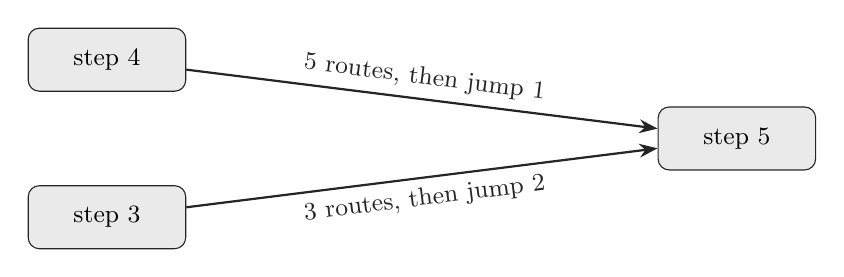
\begin{tikzpicture}[>=Stealth,every node/.style={font=\small},box/.style={draw=teal,rounded corners,minimum width=20mm,minimum height=8mm,fill=wash},arr/.style={->,thick,teal}]\node[box] (a) at (0,1) {step 4};\node[box] (b) at (0,-1) {step 3};\node[box] (c) at (8,0) {step 5};\draw[arr] (a)--node[above,sloped]{5 routes, then jump 1}(c);\draw[arr] (b)--node[below,sloped]{3 routes, then jump 2}(c);\end{tikzpicture}\end{center}\end{minipage}
\par\bigskip\begin{minipage}{\textwidth}\textbf{L1-09 / Repeated questions in the call tree}\par\begin{center}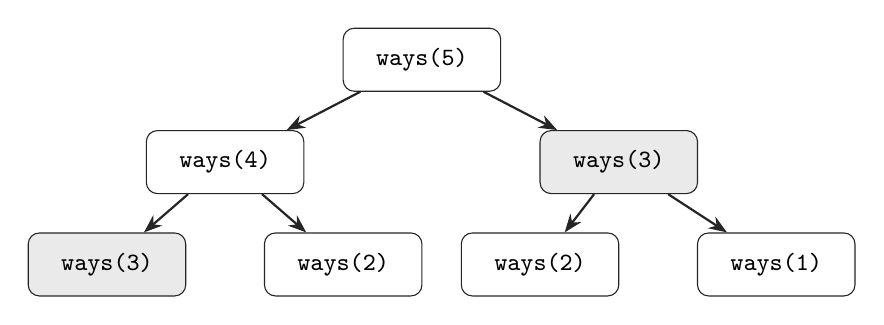
\begin{tikzpicture}[>=Stealth,every node/.style={font=\small},box/.style={draw=teal,rounded corners,minimum width=20mm,minimum height=8mm,fill=wash},arr/.style={->,thick,teal}]\node[box,fill=paper] (a) at (5,0) {\texttt{ways(5)}};\node[box,fill=paper] (b) at (2.5,-1.3) {\texttt{ways(4)}};\node[box,fill=wash] (c) at (7.5,-1.3) {\texttt{ways(3)}};\node[box,fill=wash] (d) at (1,-2.6) {\texttt{ways(3)}};\node[box,fill=paper] (e) at (4,-2.6) {\texttt{ways(2)}};\node[box,fill=paper] (f) at (6.5,-2.6) {\texttt{ways(2)}};\node[box,fill=paper] (g) at (9.5,-2.6) {\texttt{ways(1)}};\draw[arr] (a)--(b);\draw[arr] (a)--(c);\draw[arr] (b)--(d);\draw[arr] (b)--(e);\draw[arr] (c)--(f);\draw[arr] (c)--(g);\end{tikzpicture}\end{center}\end{minipage}
\par\bigskip\begin{minipage}{\textwidth}\textbf{L1-12 / Build the table in order}\par\par\medskip \begingroup\small\setlength{\tabcolsep}{4pt}\renewcommand{\arraystretch}{1.35}\begin{tabularx}{\linewidth}{>{\raggedright\arraybackslash}l>{\raggedright\arraybackslash}X>{\raggedright\arraybackslash}X>{\raggedright\arraybackslash}X>{\raggedright\arraybackslash}X>{\raggedright\arraybackslash}X>{\raggedright\arraybackslash}X}\toprule\textbf{Step} & \textbf{0} & \textbf{1} & \textbf{2} & \textbf{3} & \textbf{4} & \textbf{5}\\\midrule
ways[step] & 1 & 1 & 2 & 3 & 5 & 8\\
\bottomrule\end{tabularx}\endgroup\par\medskip \end{minipage}
\par\bigskip\begin{minipage}{\textwidth}\textbf{L1-13 / Your turn: jumps of 1 or 3}\par\par\medskip \begingroup\small\setlength{\tabcolsep}{4pt}\renewcommand{\arraystretch}{1.35}\begin{tabularx}{\linewidth}{>{\raggedright\arraybackslash}l>{\raggedright\arraybackslash}X>{\raggedright\arraybackslash}X>{\raggedright\arraybackslash}X>{\raggedright\arraybackslash}X>{\raggedright\arraybackslash}X>{\raggedright\arraybackslash}X>{\raggedright\arraybackslash}X>{\raggedright\arraybackslash}X}\toprule\textbf{Step} & \textbf{0} & \textbf{1} & \textbf{2} & \textbf{3} & \textbf{4} & \textbf{5} & \textbf{6} & \textbf{7}\\\midrule
ways[step] & 1 & 1 & 1 & 2 & 3 & 4 & 6 & 9\\
\bottomrule\end{tabularx}\endgroup\par\medskip \end{minipage}
\par\bigskip\begin{minipage}{\textwidth}\textbf{L1-15 / A greedy choice can fail}\par\par\medskip \begingroup\small\setlength{\tabcolsep}{4pt}\renewcommand{\arraystretch}{1.35}\begin{tabularx}{\linewidth}{>{\raggedright\arraybackslash}l>{\raggedright\arraybackslash}X>{\raggedright\arraybackslash}X>{\raggedright\arraybackslash}X>{\raggedright\arraybackslash}X>{\raggedright\arraybackslash}X>{\raggedright\arraybackslash}X>{\raggedright\arraybackslash}X}\toprule\textbf{Jump into stone i} & \textbf{0} & \textbf{1} & \textbf{2} & \textbf{3} & \textbf{4} & \textbf{5} & \textbf{Total}\\\midrule
heights[i] & 20 & 50 & 30 & 40 & 10 & 10 & \\
greedy 0, 2, 3, 5 & start &  & 10 & 10 &  & 30 & 50\\
best 0, 2, 4, 5 & start &  & 10 &  & 20 & 0 & 30\\
\bottomrule\end{tabularx}\endgroup\par\medskip \end{minipage}
\par\bigskip\begin{minipage}{\textwidth}\textbf{L1-18 / Frog: write the iterative solution}\par\par\medskip \begingroup\small\setlength{\tabcolsep}{4pt}\renewcommand{\arraystretch}{1.35}\begin{tabularx}{\linewidth}{>{\raggedright\arraybackslash}l>{\raggedright\arraybackslash}X>{\raggedright\arraybackslash}X>{\raggedright\arraybackslash}X>{\raggedright\arraybackslash}X>{\raggedright\arraybackslash}X>{\raggedright\arraybackslash}X}\toprule\textbf{Stone i} & \textbf{0} & \textbf{1} & \textbf{2} & \textbf{3} & \textbf{4} & \textbf{5}\\\midrule
heights[i] & 20 & 50 & 30 & 40 & 10 & 10\\
best[i] & 0 & 30 & 10 & 20 & 30 & 30\\
\bottomrule\end{tabularx}\endgroup\par\medskip \end{minipage}
\par\bigskip\begin{minipage}{\textwidth}\textbf{L1-19 / Your turn: a new Frog instance}\par\par\medskip \begingroup\small\setlength{\tabcolsep}{4pt}\renewcommand{\arraystretch}{1.35}\begin{tabularx}{\linewidth}{>{\raggedright\arraybackslash}X>{\raggedright\arraybackslash}X>{\raggedright\arraybackslash}X>{\raggedright\arraybackslash}X>{\raggedright\arraybackslash}X}\toprule\textbf{Stone i} & \textbf{0} & \textbf{1} & \textbf{2} & \textbf{3}\\\midrule
heights[i] & 10 & 30 & 20 & 40\\
best[i] & 0 & 20 & 10 & 30\\
\bottomrule\end{tabularx}\endgroup\par\medskip \end{minipage}
\par\bigskip\begin{minipage}{\textwidth}\textbf{L1-21 / Frog: recover a cheapest path}\par\par\medskip \begingroup\small\setlength{\tabcolsep}{4pt}\renewcommand{\arraystretch}{1.35}\begin{tabularx}{\linewidth}{>{\raggedright\arraybackslash}l>{\raggedright\arraybackslash}X>{\raggedright\arraybackslash}X>{\raggedright\arraybackslash}X>{\raggedright\arraybackslash}X>{\raggedright\arraybackslash}X>{\raggedright\arraybackslash}X}\toprule\textbf{Stone i} & \textbf{0} & \textbf{1} & \textbf{2} & \textbf{3} & \textbf{4} & \textbf{5}\\\midrule
heights[i] & 20 & 50 & 30 & 40 & 10 & 10\\
best[i] & 0 & 30 & 10 & 20 & 30 & 30\\
previous[i] & -1 & 0 & 0 & 2 & 2 & 4\\
\bottomrule\end{tabularx}\endgroup\par\medskip \end{minipage}
\Needspace{18\baselineskip}\textbf{Frog as a graph / L1-16 and L1-21}\par This has the same forward connections as the staircase with moves of one or two steps. Staircase counts all routes. Frog attaches a cost to each arrow and asks for a route whose total cost is smallest. The horizontal position is the stone index, not its height; a fall in height still costs energy.\par\medskip\resizebox{\linewidth}{!}{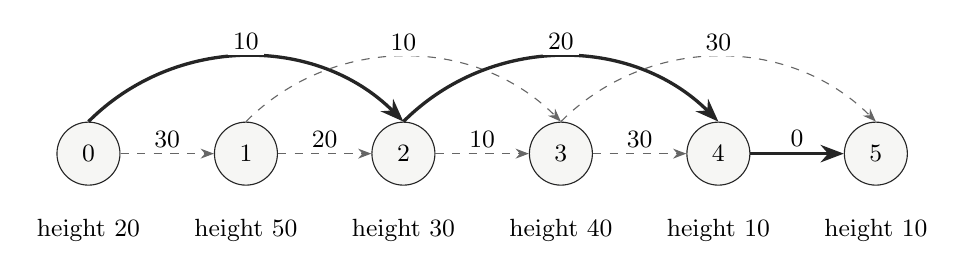
\begin{tikzpicture}[x=1cm,y=1cm,>=Stealth,every node/.style={font=\small}]
\node[draw=ink,circle,minimum size=8mm,fill=codepaper] (g0) at (0,0) {0};
\node[below=3mm] at (g0.south) {height 20};
\node[draw=ink,circle,minimum size=8mm,fill=codepaper] (g1) at (2,0) {1};
\node[below=3mm] at (g1.south) {height 50};
\node[draw=ink,circle,minimum size=8mm,fill=codepaper] (g2) at (4,0) {2};
\node[below=3mm] at (g2.south) {height 30};
\node[draw=ink,circle,minimum size=8mm,fill=codepaper] (g3) at (6,0) {3};
\node[below=3mm] at (g3.south) {height 40};
\node[draw=ink,circle,minimum size=8mm,fill=codepaper] (g4) at (8,0) {4};
\node[below=3mm] at (g4.south) {height 10};
\node[draw=ink,circle,minimum size=8mm,fill=codepaper] (g5) at (10,0) {5};
\node[below=3mm] at (g5.south) {height 10};
\draw[->,draw=quiet,dashed] (g0.east) -- node[above,fill=white,inner sep=2pt] {30} (g1.west);
\draw[->,very thick,draw=ink] (g0.north) to[bend left=45] node[above,fill=white,inner sep=2pt] {10} (g2.north);
\draw[->,draw=quiet,dashed] (g1.east) -- node[above,fill=white,inner sep=2pt] {20} (g2.west);
\draw[->,draw=quiet,dashed] (g1.north) to[bend left=45] node[above,fill=white,inner sep=2pt] {10} (g3.north);
\draw[->,draw=quiet,dashed] (g2.east) -- node[above,fill=white,inner sep=2pt] {10} (g3.west);
\draw[->,very thick,draw=ink] (g2.north) to[bend left=45] node[above,fill=white,inner sep=2pt] {20} (g4.north);
\draw[->,draw=quiet,dashed] (g3.east) -- node[above,fill=white,inner sep=2pt] {30} (g4.west);
\draw[->,draw=quiet,dashed] (g3.north) to[bend left=45] node[above,fill=white,inner sep=2pt] {30} (g5.north);
\draw[->,very thick,draw=ink] (g4.east) -- node[above,fill=white,inner sep=2pt] {0} (g5.west);
\end{tikzpicture}}\par Solid arrows recover 0, 2, 4, 5 at cost 30; dashed arrows are other legal jumps. The graph has one node per stone. A recursion tree shows calls: several branches may ask for the cheapest cost to stone 2. Those calls refer to the same graph node. Caching merges their repeated work. Iteration visits nodes from left to right: every incoming arrow then comes from a stone whose best cost is already known.
\topicflow{CODE ANSWERS}{Complete code}
Every function used in class, in question order. Line numbers are the same as in the tutor book.\par\medskip
\Needspace{13\baselineskip}
{\color{teal}\textbf{L1-03}}\quad\textbf{\texttt{power2}}\label{L1-code-power2}\par
\begin{lstlisting}[style=numbered]
def power2(n):
    if n == 0:
        return 1
    return 2 * power2(n - 1)
\end{lstlisting}

\begin{lstlisting}
print(power2(3))
\end{lstlisting}
\textbf{Expected output:} 8
\par\bigskip
\Needspace{13\baselineskip}
{\color{teal}\textbf{L1-04}}\quad\textbf{\texttt{factorial}}\label{L1-code-factorial}\par
\begin{lstlisting}[style=numbered]
def factorial(n):
    if n == 0:
        return 1
    return n * factorial(n - 1)
\end{lstlisting}

\begin{lstlisting}
print([factorial(n) for n in range(6)])
\end{lstlisting}
\textbf{Expected output:} [1, 1, 2, 6, 24, 120]
\par\bigskip
\Needspace{18\baselineskip}
{\color{teal}\textbf{L1-08}}\quad\textbf{\texttt{stairs\_slow}}\label{L1-code-stairs_slow}\par
\begin{lstlisting}[style=numbered]
def stairs_slow(n):
    if n < 0:
        return 0
    if n == 0:
        return 1
    return stairs_slow(n - 1) + stairs_slow(n - 2)
\end{lstlisting}
\textbf{Recursion depth.} Python stops recursion at about 1,000 nested calls by default, so this recursive version is for small inputs and the small and edge test files only. Use the iterative version for the medium and large files.


\begin{lstlisting}
print(stairs_slow(5))
\end{lstlisting}
\textbf{Expected output:} 8
\par\bigskip
\Needspace{21\baselineskip}
{\color{teal}\textbf{L1-10}}\quad\textbf{\texttt{stairs\_cached}}\label{L1-code-stairs_cached}\par
\begin{lstlisting}[style=numbered]
def stairs_cached(n):
    cache = {0: 1}
    def ways(step):
        if step < 0:
            return 0
        if step not in cache:
            cache[step] = ways(step - 1) + ways(step - 2)
        return cache[step]
    return ways(n)
\end{lstlisting}
\textbf{Recursion depth.} Python stops recursion at about 1,000 nested calls by default, so this recursive version is for small inputs and the small and edge test files only. Use the iterative version for the medium and large files.


\begin{lstlisting}
print(stairs_cached(20))
\end{lstlisting}
\textbf{Expected output:} 10946
\par\bigskip
\Needspace{21\baselineskip}
{\color{teal}\textbf{L1-11}}\quad\textbf{\texttt{recursion\_demo}}\label{L1-code-recursion_demo}\par
\begin{lstlisting}[style=numbered]
import sys

def recursion_demo():
    def descend(n):
        if n == 0:
            return 0
        return 1 + descend(n - 1)
    try:
        descend(sys.getrecursionlimit() + 10)
    except RecursionError:
        return 'Caught RecursionError: too many nested calls.'
    return 'No RecursionError: the limit was not reached.'
\end{lstlisting}

\begin{lstlisting}
print(recursion_demo())
\end{lstlisting}
\textbf{Expected output:} Caught RecursionError: too many nested calls.
\par\bigskip
\Needspace{17\baselineskip}
{\color{teal}\textbf{L1-12}}\quad\textbf{\texttt{stairs\_table}}\label{L1-code-stairs_table}\par
\begin{lstlisting}[style=numbered]
def stairs_table(n):
    ways = [0] * (n + 1)
    ways[0] = 1
    for step in range(1, n + 1):
        ways[step] = ways[step - 1]
        if step >= 2:
            ways[step] += ways[step - 2]
    return ways[n]
\end{lstlisting}

\begin{lstlisting}
print([stairs_table(n) for n in range(6)])
\end{lstlisting}
\textbf{Expected output:} [1, 1, 2, 3, 5, 8]
\par\bigskip
\Needspace{17\baselineskip}
{\color{teal}\textbf{L1-13}}\quad\textbf{\texttt{stairs\_13}}\label{L1-code-stairs_13}\par
\begin{lstlisting}[style=numbered]
def stairs_13(n):
    ways = [0] * (n + 1)
    ways[0] = 1
    for step in range(1, n + 1):
        for jump in (1, 3):
            if step >= jump:
                ways[step] += ways[step - jump]
    return ways[n]
\end{lstlisting}

\begin{lstlisting}
print([stairs_13(n) for n in range(8)])
\end{lstlisting}
\textbf{Expected output:} [1, 1, 1, 2, 3, 4, 6, 9]
\par\bigskip
\Needspace{22\baselineskip}
{\color{teal}\textbf{L1-16}}\quad\textbf{\texttt{frog\_slow}}\label{L1-code-frog_slow}\par
\begin{lstlisting}[style=numbered]
def frog_slow(heights):
    def cost(i):
        if i == 0:
            return 0
        one = cost(i - 1) + abs(heights[i] - heights[i - 1])
        if i == 1:
            return one
        two = cost(i - 2) + abs(heights[i] - heights[i - 2])
        return min(one, two)
    return cost(len(heights) - 1)
\end{lstlisting}
\textbf{Recursion depth.} Python stops recursion at about 1,000 nested calls by default, so this recursive version is for small inputs and the small and edge test files only. Use the iterative version for the medium and large files.


\begin{lstlisting}
print(frog_slow([20, 50, 30, 40, 10, 10]))
\end{lstlisting}
\textbf{Expected output:} 30
\par\bigskip
\Needspace{24\baselineskip}
{\color{teal}\textbf{L1-17}}\quad\textbf{\texttt{frog\_cached}}\label{L1-code-frog_cached}\par
\begin{lstlisting}[style=numbered]
def frog_cached(heights):
    cache = {0: 0}
    def cost(i):
        if i not in cache:
            one = cost(i - 1) + abs(heights[i] - heights[i - 1])
            answer = one
            if i >= 2:
                two = cost(i - 2) + abs(heights[i] - heights[i - 2])
                answer = min(one, two)
            cache[i] = answer
        return cache[i]
    return cost(len(heights) - 1)
\end{lstlisting}
\textbf{Recursion depth.} Python stops recursion at about 1,000 nested calls by default, so this recursive version is for small inputs and the small and edge test files only. Use the iterative version for the medium and large files.


\begin{lstlisting}
print(frog_cached([20, 50, 30, 40, 10, 10]))
\end{lstlisting}
\textbf{Expected output:} 30
\par\bigskip
\Needspace{17\baselineskip}
{\color{teal}\textbf{L1-18}}\quad\textbf{\texttt{frog\_table}}\label{L1-code-frog_table}\par
\begin{lstlisting}[style=numbered]
def frog_table(heights):
    best = [0] * len(heights)
    for i in range(1, len(heights)):
        best[i] = best[i - 1] + abs(heights[i] - heights[i - 1])
        if i >= 2:
            two = best[i - 2] + abs(heights[i] - heights[i - 2])
            best[i] = min(best[i], two)
    return best[-1]
\end{lstlisting}

\begin{lstlisting}
print(frog_table([20, 50, 30, 40, 10, 10]))
\end{lstlisting}
\textbf{Expected output:} 30
\par\bigskip
\Needspace{28\baselineskip}
{\color{teal}\textbf{L1-21}}\quad\textbf{\texttt{frog\_path}}\label{L1-code-frog_path}\par
\begin{lstlisting}[style=numbered]
def frog_path(heights):
    n = len(heights)
    best = [0] * n
    previous = [-1] * n
    for i in range(1, n):
        best[i] = best[i - 1] + abs(heights[i] - heights[i - 1])
        previous[i] = i - 1
        if i >= 2:
            two = best[i - 2] + abs(heights[i] - heights[i - 2])
            if two < best[i]:
                best[i] = two
                previous[i] = i - 2
    path = []
    i = n - 1
    while i != -1:
        path.append(i)
        i = previous[i]
    path.reverse()
    return best[-1], path
\end{lstlisting}

\begin{lstlisting}
print(frog_path([20, 50, 30, 40, 10, 10]))
\end{lstlisting}
\textbf{Expected output:} (30, [0, 2, 4, 5])
\par\bigskip
\topicflow{EXERCISE CHECKS}{Expected notebook results}
\Needspace{8\baselineskip}\textbf{L1-13 / stairs\_13}\par
Use the complete \texttt{stairs\_13} solution on page~\pageref{L1-code-stairs_13}. The function name and parameters are the same in the notebook.

\begin{lstlisting}
stairs_13(0)  # expected: 1
stairs_13(2)  # expected: 1
stairs_13(7)  # expected: 9
\end{lstlisting}
\Needspace{8\baselineskip}\textbf{L1-18 / frog\_table}\par
Use the complete \texttt{frog\_table} solution on page~\pageref{L1-code-frog_table}. The function name and parameters are the same in the notebook.

\begin{lstlisting}
frog_table([20, 50, 30, 40, 10, 10])  # expected: 30
frog_table([10, 30])                  # expected: 20
\end{lstlisting}
\Needspace{8\baselineskip}\textbf{L1-19 / frog\_table}\par
Use the complete \texttt{frog\_table} solution on page~\pageref{L1-code-frog_table}. The function name and parameters are the same in the notebook.

\begin{lstlisting}
frog_table([10, 30, 20, 40])          # expected: 30
frog_table([20, 50, 30, 40, 10, 10])  # expected: 30
frog_table([7] * 100000)              # expected: 0
\end{lstlisting}
\Needspace{8\baselineskip}\textbf{L1-21 / frog\_path}\par
Use the complete \texttt{frog\_path} solution on page~\pageref{L1-code-frog_path}. The function name and parameters are the same in the notebook.

\begin{lstlisting}
frog_path([20, 50, 30, 40, 10, 10])  # expected: (30, [0, 2, 4, 5])
frog_path([10, 30, 20, 40])          # expected: (30, [0, 2, 3])
frog_path([7, 7, 7])                 # expected: (0, [0, 1, 2])
frog_path([7])                       # expected: (0, [0])
\end{lstlisting}
\clearpage\renewcommand{\lessonnumber}{2}\renewcommand{\lessonheading}{Lesson 2 · Dice Combinations and Grid Paths}\phantomsection\label{lesson-2}\pdfbookmark[-1]{Lesson 2: Dice Combinations and Grid Paths}{lesson-2-bookmark}
\noindent\makebox[\linewidth][l]{\begin{minipage}{176mm}{\heavy\fontsize{23}{28}\selectfont\raggedright Lesson 2\par}\vspace{2mm}{\heavy\fontsize{19}{24}\selectfont\raggedright Dice Combinations and Grid Paths\par}\end{minipage}}\par\vspace{5mm}
\href{https://colab.research.google.com/github/fifteen02/julians-pathfinder/blob/main/Lesson\%202/lesson.ipynb}{\underline{Open this lesson in Google Colab}}\par
\topicflow{BEFORE CLASS}{The lesson route}
\par\noindent\colorbox{wash}{\parbox{\dimexpr\linewidth-2\fboxsep\relax}{\vspace{3pt}{\color{quiet}\heavy\fontsize{8.5}{10}\selectfont MAIN IDEA: SAY THIS AT THE START}\par\smallskip{\heavy\fontsize{15}{18}\selectfont Count the ways to arrive.}\par\smallskip To count the ways to reach a target, split them by their last move and add the counts for where that move started.\par\medskip\textbf{By the end of the lesson you will be able to}\begin{itemize}\item count dice sequences for a total by grouping them by their last number;\item explain why the empty sequence counts 1 and why remainders keep big counts small;\item count paths through a grid with blocked cells, from above and from the left.\end{itemize}\vspace{3pt}}}\par

The target is understanding, not finishing every page. Use the question IDs to move between slides, worksheet and notebook. Questions labelled optional are extensions.

\begingroup\small\setlength{\tabcolsep}{4pt}\renewcommand{\arraystretch}{1.35}\begin{tabularx}{\linewidth}{>{\raggedright\arraybackslash}p{18mm}>{\raggedright\arraybackslash}X>{\raggedright\arraybackslash}p{38mm}}\toprule\textbf{Minutes} & \textbf{Activity} & \textbf{Question IDs}\\\midrule
0-10 & Recall: what are we storing? & L2-01\\
10-20 & A total of three; six possible last numbers & L2-02 to L2-03\\
20-45 & Dice: recursion and caching, then fill the totals in order & L2-04 to L2-05\\
45-60 & Why take a remainder? Your turn: three faces & L2-06 to L2-07\\
60-65 & Break & \\
65-75 & Grid Paths: draw routes, then two counts per cell & L2-09 to L2-10\\
75-95 & Grid recursion, then grid iteration & L2-11 to L2-12\\
95-105 & Your turn: test the boundaries & L2-13\\
105-115 & Exit question: the shared counting idea & L2-14\\
115-120 & Optional buffer preview (full trace next session) & L2-08\\
\bottomrule\end{tabularx}\endgroup

\labeltext{Pacing and preparation}
Ask students to predict before running code. Allow a quiet individual attempt before asking for a volunteer. If an answer is wrong, trace the first state where it differs. Keep the final ten minutes for explanation and questions. Move an unfinished implementation to the next session rather than shortening the reasoning.

Students need Python functions, lists, loops, indexing, comparisons and basic arithmetic. Introduce new syntax beside the program that uses it. Use small inputs for uncached recursion; the notebook never starts an enormous recursive run. Python stops recursion at about 1,000 nested calls by default, so every recursive version in this lesson, cached or not, is for small inputs and the small and edge test files only. The medium and large files are for the iterative versions.

The final five minutes can introduce L2-08: why only six Dice counts are needed. Allow 15-20 minutes in a follow-up to trace the circular buffer and running sum in full.

Open lesson.ipynb in Jupyter or upload it to Google Colab, choose a Python 3 runtime, and run the setup cell first. Shift+Enter runs a cell. Restart and run from the top if names or data become stale. The notebook needs only Python standard-library features and no local files.
\topic{KEEP BESIDE YOUR WORK}{The route and the rules}
\textbf{Our route}\par Count ordered dice sequences by their final number. Try recursion, save repeated answers, then fill a table. Then see how six reused entries reduce Dice memory from O(n) to O(1), with an optional running sum. Afterwards count grid paths by their final move. The full Dice table remains useful for learning; the buffer is a memory improvement.\par\medskip
\textbf{Dice rules · L2-02 to L2-08}\par Choose any finite ordered sequence of values from 1 to 6. Count sequences whose total is exactly the target n. There is no fixed number of throws and no probability calculation. [1, 2] and [2, 1] are different sequences. For L2-07 only, allow 1, 2 and 3.\par\medskip
\textbf{Large counts}\par The final iterative dice and grid programs return the remainder after dividing the count by 1,000,000,007. Python writes this as \texttt{count \% 1\_000\_000\_007}. Small examples on these sheets are below that number, so their counts are unchanged. L2-06 explains why taking remainders during the calculation is valid.\par\medskip
\textbf{Grid rules · L2-09 to L2-14}\par The grid has n rows and n columns, numbered from 0. A dot means an open cell; a star means a blocked cell. Start at row 0, column 0. Reach row n - 1, column n - 1 using moves of one cell right or one cell down. A path may never enter a blocked cell.\par\medskip
\textbf{Names used in the questions}\par \texttt{ways[total]} stores the number of sequences whose sum is that total. \texttt{paths[r][c]} stores the number of paths to row r, column c. The indices identify a total or a cell; the stored values count sequences or paths. A recursive function answers the same question by asking about smaller totals or earlier cells.\par\medskip
\topicflow{IN CLASS}{Questions, answers and prompts}
\markboth{Dice: count ordered sequences}{}{\color{quiet}\heavy\fontsize{10}{13}\selectfont DICE: COUNT ORDERED SEQUENCES}\par\medskip
\noindent\begin{minipage}{\textwidth}
{\color{teal}\textbf{L2-01}}\quad \textbf{Recall: what are we storing?}\par\smallskip
\textbf{Ask.} In staircase, what does ways[4] = 5 mean? In Frog, what does best[4] = 30 mean? Which problem adds and which takes a minimum?\par\smallskip
\textbf{Answer.} There are 5 routes to step 4. The cheapest Frog route to stone 4 costs 30. Staircase adds counts from separate groups; Frog takes the minimum of competing total costs.\par\smallskip
\textbf{Prompt if stuck.} Say whether the stored number counts routes or measures a route cost.\par\smallskip
\textbf{Watch for.} The index is not the answer.
\end{minipage}\par\medskip{\color{lightink}\hrule height .4pt}\medskip

\noindent\begin{minipage}{\textwidth}
{\color{teal}\textbf{L2-02}}\quad \textbf{A total of three}\par\smallskip
\textbf{Ask.} List every ordered sequence of numbers from 1 to 6 whose sum is exactly 3. What happens to sequences containing a 4, 5 or 6?\par\smallskip
\textbf{Answer.} The four sequences are [3], [1, 2], [2, 1] and [1, 1, 1]. A sequence containing 4, 5 or 6 already exceeds the target. We count valid sequences rather than simulate random throws.\par\smallskip
\textbf{Prompt if stuck.} Choose the last number, then ask what total remains.\par\smallskip
\textbf{Watch for.} Unordered partitions count [1, 2] only once and solve a different problem.
\end{minipage}\par\medskip{\color{lightink}\hrule height .4pt}\medskip

\noindent\begin{minipage}{\textwidth}
{\color{teal}\textbf{L2-03}}\quad \textbf{Six possible last numbers}\par\smallskip
\textbf{Ask.} Let ways[total] count ordered sequences of values 1 to 6 whose sum is that total. Explain ways[0] = 1. For target 4, group sequences by their last number and add the earlier counts. Copy your L2-02 count into total 3, then fill totals 5, 6 and 7 in the table.\par\smallskip
\textbf{Answer.} The empty sequence is the one sequence with total 0. For total 4, final numbers 1, 2, 3 and 4 give counts 4 + 2 + 1 + 1 = 8. Totals 5 and 6 give 16 and 32. Total 7 uses totals 6 through 1: 32 + 16 + 8 + 4 + 2 + 1 = 63.\par\smallskip
\textbf{Prompt if stuck.} Take the sequence [1, 2, 1] with total 4 and remove its last number. What total is left? How many sequences have that total?\par\smallskip
\textbf{Watch for.} Adding an extra 1 after the sum counts a route twice; ways[0] already handles a single throw.
\end{minipage}\par\medskip{\color{lightink}\hrule height .4pt}\medskip

\noindent\begin{minipage}{\textwidth}
{\color{teal}\textbf{L2-04}}\quad \textbf{Dice: recursion, then caching}\par\smallskip
\textbf{Ask.} Write dice\_slow(n) recursively to count ordered sequences of faces 1 to 6 with total n. Trace target 4. Then write dice\_cached(n), adding a cache: which input identifies a repeated question? Use the uncached version only on tiny targets. In the cached version, store counts modulo 1,000,000,007.\par\smallskip
\par\smallskip{\small\textbf{Students start with:}}\par\smallskip\noindent\colorbox{codepaper}{\parbox{\dimexpr\linewidth-2\fboxsep\relax}{\small\ttfamily\raggedright def dice\_slow(n):\\\hspace*{2.4em}return None  \# Replace with your answer.\\\mbox{}\\def dice\_cached(n):\\\hspace*{2.4em}def count(total):\\\hspace*{4.8em}return None  \# Your helper goes here.\\\hspace*{2.4em}return count(n)}}\par
{\small\textbf{What each function returns.}\par dice\_slow(n): the exact number of ordered dice sequences with total n.\par dice\_cached(n): the count for total n, modulo 1,000,000,007.\par count(total): the count for this total, modulo 1,000,000,007.\par }
{\small\textbf{Hints to give, one at a time.}}\begin{itemize}\item What is the count for total 0?\item Which faces can be the last one when the remaining total is small?\item What input identifies a repeated question, and where must the saved answers live so that every call shares them?\end{itemize}
\textbf{Answer.} Use one cache key per target total. Total 0 contributes 1. For a positive total, try each final face that fits and add the counts for the smaller targets. Faces larger than the remaining total are skipped, so no negative total is ever asked. Target 4 returns 8. A repeated target reads its saved answer instead of branching again.\par\smallskip
\textbf{Prompt if stuck.} Keep the dictionary outside the nested recursive function.\par\smallskip
\textbf{Watch for.} Caching is valid because the allowed faces remain fixed throughout one call.\par\smallskip Full code: \texttt{dice\_slow} (page~\pageref{L2-code-dice_slow}), \texttt{dice\_cached} (page~\pageref{L2-code-dice_cached}).
\end{minipage}\par\medskip{\color{lightink}\hrule height .4pt}\medskip

\noindent\begin{minipage}{\textwidth}
{\color{teal}\textbf{L2-05}}\quad \textbf{Dice: fill the totals in order}\par\smallskip
\textbf{Ask.} Write dice\_table(n) using a loop. Store in ways[total] the count for that total, modulo 1,000,000,007. Fill totals from 1 upwards. When the loop reaches total 7, which earlier totals does it read? Add their counts and explain the result.\par\smallskip
\par\smallskip{\small\textbf{Students start with:}}\par\smallskip\noindent\colorbox{codepaper}{\parbox{\dimexpr\linewidth-2\fboxsep\relax}{\small\ttfamily\raggedright def dice\_table(n):\\\hspace*{2.4em}return None  \# Replace with your answer.}}\par
{\small\textbf{What each function returns.}\par dice\_table(n): the number of ordered dice sequences with total n, modulo 1,000,000,007.\par }
{\small\textbf{Hints to give, one at a time.}}\begin{itemize}\item Which entry is known before the loop?\item For each total, which earlier totals can the last face come from?\item Where do you take the remainder so that stored numbers stay small?\end{itemize}
\textbf{Answer.} Total 7 reads counts for totals 6, 5, 4, 3, 2 and 1. Their sum is 32 + 16 + 8 + 4 + 2 + 1 = 63. Fill totals from 1 upwards, starting with ways[0] = 1.\par\smallskip
\textbf{Prompt if stuck.} The new answer is the sum of valid earlier answers, not an earlier answer plus one.\par\smallskip
\textbf{Watch for.} Do not fill a list with zeros and forget the one empty sequence.\par\smallskip Full code: \texttt{dice\_table} (page~\pageref{L2-code-dice_table}).
\end{minipage}\par\medskip{\color{lightink}\hrule height .4pt}\medskip

\noindent\begin{minipage}{\textwidth}
{\color{teal}\textbf{L2-06}}\quad \textbf{Why take a remainder?}\par\smallskip
\textbf{Ask.} Modulo 7 means the remainder after division by 7. Compare (12 + 13) \% 7 with ((12 \% 7) + (13 \% 7)) \% 7. Why do both calculations give the same remainder? How does this help when dice counts become very large?\par\smallskip
\textbf{Answer.} 12 + 13 = 25, whose remainder is 4. Separately, 12 has remainder 5 and 13 has remainder 6; 5 + 6 = 11 also has remainder 4. Removing whole multiples of 7 does not change a remainder modulo 7. Dice uses the same rule with 1,000,000,007 to keep stored numbers small.\par\smallskip
\textbf{Prompt if stuck.} Write 12 = 7 + 5 and 13 = 7 + 6. Which parts can you throw away without changing the remainder of the sum?\par\smallskip
\textbf{Watch for.} The modulo operation is not a probability and does not count only a subset of sequences.
\end{minipage}\par\medskip{\color{lightink}\hrule height .4pt}\medskip

\noindent\begin{minipage}{\textwidth}
{\color{teal}\textbf{L2-07}}\quad \textbf{Your turn: three faces}\par\smallskip
\textbf{Ask.} Write dice\_123(n) by adapting dice\_table from L2-05 to allow only faces 1, 2 and 3. First fill counts for totals 0 through 5, then write and test your code. Explain the answer for total 5.\par\smallskip
\par\smallskip{\small\textbf{Students start with:}}\par\smallskip\noindent\colorbox{codepaper}{\parbox{\dimexpr\linewidth-2\fboxsep\relax}{\small\ttfamily\raggedright def dice\_123(n):\\\hspace*{2.4em}return None  \# Replace with your answer.}}\par
{\small\textbf{What each function returns.}\par dice\_123(n): the number of ordered sequences of 1, 2 and 3 with total n, modulo 1,000,000,007.\par }
{\small\textbf{Hints to give, one at a time.}}\begin{itemize}\item Which part of dice\_table depends on the faces allowed?\item Check total 4 by hand before you run the code.\end{itemize}
\textbf{Answer.} The counts are [1, 1, 2, 4, 7, 13]. Total 5 combines totals 4, 3 and 2, giving 7 + 4 + 2 = 13. Only the allowed-face loop changes.\par\smallskip
\textbf{Prompt if stuck.} Group routes by final face 1, 2 or 3.\par\smallskip
\textbf{Watch for.} Changing the allowed faces must not change ways[0].\par\smallskip Full code: \texttt{dice\_123} (page~\pageref{L2-code-dice_123}).
\end{minipage}\par\medskip{\color{lightink}\hrule height .4pt}\medskip

\Needspace{14\baselineskip}\markboth{Optional: reuse six counts}{}{\color{quiet}\heavy\fontsize{10}{13}\selectfont OPTIONAL: REUSE SIX COUNTS}\par\medskip
\noindent\begin{minipage}{\textwidth}
{\color{teal}\textbf{L2-08 / OPTIONAL}}\quad \textbf{Extension: six slots instead of a full table}\par\smallskip
\textbf{Ask.} Before total 7, recent is [32, 1, 2, 4, 8, 16] in slots 0 to 5. These store counts for totals [6, 1, 2, 3, 4, 5]. The running sum window is 63. Which slot does 7 \% 6 choose, and which old count must be saved before overwriting it? Store the answer for total 7, then prepare the next sum. What should dice\_window(7) return? Explain why six slots are enough.\par\smallskip
\textbf{Answer.} 7 \% 6 chooses slot 1. Save its old count 1, then store 63. Prepare the next sum: 63 - 1 + 63 = 125, for total 8. Return recent[1] = 63. Only the six preceding counts are needed: reusing their slots reduces memory from O(n) to O(1). Time remains O(n).\par\smallskip
\textbf{Prompt if stuck.} Separate the total, its slot and the count stored there. Save the old count, write the current answer, then prepare the next sum.\par\smallskip
\textbf{Watch for.} Slot 1 can hold the count for total 1 or total 7 at different times. The updated running sum answers the next total.\par\smallskip Full code: \texttt{dice\_ring} (page~\pageref{L2-code-dice_ring}), \texttt{dice\_window} (page~\pageref{L2-code-dice_window}).
\end{minipage}\par\medskip{\color{lightink}\hrule height .4pt}\medskip

\Needspace{14\baselineskip}\markboth{Grid Paths: count routes to each cell}{}{\color{quiet}\heavy\fontsize{10}{13}\selectfont GRID PATHS: COUNT ROUTES TO EACH CELL}\par\medskip
\noindent\begin{minipage}{\textwidth}
{\color{teal}\textbf{L2-09}}\quad \textbf{Grid Paths: draw before coding}\par\smallskip
\textbf{Ask.} In a 3 by 3 grid, a dot is open and a star is blocked. Start at the top left and finish at the bottom right. Move only one cell right or down. The centre cell is blocked. Draw or list every legal route; how many are there?\par\smallskip
\textbf{Answer.} Two routes remain: right, right, down, down; and down, down, right, right. Every other route would visit the blocked centre square.\par\smallskip
\textbf{Prompt if stuck.} Trace the two routes along the outside edges.\par\smallskip
\textbf{Watch for.} Counting a path that passes through the centre breaks the obstacle rule.
\end{minipage}\par\medskip{\color{lightink}\hrule height .4pt}\medskip

\noindent\begin{minipage}{\textwidth}
{\color{teal}\textbf{L2-10}}\quad \textbf{A grid cell receives two counts}\par\smallskip
\textbf{Ask.} Rows and columns are numbered from 0. Let paths[r][c] count routes from the top-left cell to row r, column c. From which cells can the last move arrive? Fill the count table for the 3 by 3 grid with its centre blocked, writing 0 for the blocked cell.\par\smallskip
\textbf{Answer.} An open cell receives paths from above and from its left. The count table is rows [1, 1, 1], [1, 0, 1], [1, 1, 2]. A blocked cell contributes zero.\par\smallskip
\textbf{Prompt if stuck.} At the bottom-right cell, the two neighbour counts are both 1.\par\smallskip
\textbf{Watch for.} A blocked cell is zero even when its neighbours have positive counts.
\end{minipage}\par\medskip{\color{lightink}\hrule height .4pt}\medskip

\noindent\begin{minipage}{\textwidth}
{\color{teal}\textbf{L2-11}}\quad \textbf{Grid recursion identifies a cell}\par\smallskip
\textbf{Ask.} Write grid\_cached(rows) with a cached recursive helper count(r, c). The helper returns the number of legal paths from the top-left cell to cell (r, c). Ask about the cells above and to the left. State the answers for an outside cell, a blocked cell and an open starting cell. Why do the calls stop?\par\smallskip
\par\smallskip{\small\textbf{Students start with:}}\par\smallskip\noindent\colorbox{codepaper}{\parbox{\dimexpr\linewidth-2\fboxsep\relax}{\small\ttfamily\raggedright def grid\_cached(rows):\\\hspace*{2.4em}n = len(rows)\\\hspace*{2.4em}def count(r, c):\\\hspace*{4.8em}return None  \# Your helper goes here.\\\hspace*{2.4em}return count(n - 1, n - 1)}}\par
{\small\textbf{What each function returns.}\par grid\_cached(rows): the number of legal paths from top-left to bottom-right, modulo 1,000,000,007.\par count(r, c): the number of legal paths from top-left to cell (r, c), modulo 1,000,000,007.\par }
{\small\textbf{Hints to give, one at a time.}}\begin{itemize}\item Which cells can you answer directly: outside the grid, blocked, and the start?\item From which two cells can the last move into (r, c) come?\end{itemize}
\textbf{Answer.} The key is the pair (r, c). Each call goes one row up or one column left, so r + c decreases. Outside cells and blocked cells return 0; the open starting cell returns 1.\par\smallskip
\textbf{Prompt if stuck.} The row alone cannot identify a cell.\par\smallskip
\textbf{Watch for.} Caching only r would mix cells in different columns.\par\smallskip Full code: \texttt{grid\_slow} (page~\pageref{L2-code-grid_slow}), \texttt{grid\_cached} (page~\pageref{L2-code-grid_cached}).
\end{minipage}\par\medskip{\color{lightink}\hrule height .4pt}\medskip

\noindent\begin{minipage}{\textwidth}
{\color{teal}\textbf{L2-12}}\quad \textbf{Grid iteration and independent rows}\par\smallskip
\textbf{Ask.} Write grid\_table(rows) using loops over rows and columns. The grid has n rows and n columns. Fill paths[r][c], taking counts modulo 1,000,000,007. Why does [[0] * n for \_ in range(n)] create independent rows? For n = 2, show what goes wrong with [[0] * n] * n when one cell changes.\par\smallskip
\par\smallskip{\small\textbf{Students start with:}}\par\smallskip\noindent\colorbox{codepaper}{\parbox{\dimexpr\linewidth-2\fboxsep\relax}{\small\ttfamily\raggedright def grid\_table(rows):\\\hspace*{2.4em}return None  \# Replace with your answer.}}\par
{\small\textbf{What each function returns.}\par grid\_table(rows): the number of legal paths from top-left to bottom-right, modulo 1,000,000,007.\par }
{\small\textbf{Hints to give, one at a time.}}\begin{itemize}\item Create the table so that every row is a separate list.\item In which order must you visit the cells so that the cells above and to the left are already filled?\item What does a blocked cell store?\end{itemize}
\textbf{Answer.} A comprehension builds a new list for each row. With bad = [[0] * 2] * 2, setting bad[0][0] = 1 makes both rows [1, 0], because they share one list. Separate rows keep the second row unchanged. Fill each open cell from above and left, then return the bottom-right count.\par\smallskip
\textbf{Prompt if stuck.} Try creating a 2 by 2 table and setting only its top-left entry.\par\smallskip
\textbf{Watch for.} List multiplication copies references, not nested row objects.\par\smallskip Full code: \texttt{grid\_table} (page~\pageref{L2-code-grid_table}).
\end{minipage}\par\medskip{\color{lightink}\hrule height .4pt}\medskip

\noindent\begin{minipage}{\textwidth}
{\color{teal}\textbf{L2-13}}\quad \textbf{Your turn: test the boundaries}\par\smallskip
\textbf{Ask.} Test your grid\_table(rows) from L2-12. First predict the answers for a single open cell, a single blocked cell, an open 2 by 2 grid, and a 3 by 3 grid with the centre blocked. Then run your function and compare.\par\smallskip
\textbf{Answer.} The answers are 1, 0, 2 and 2 respectively. An open start has one empty route. A blocked start has none. In the 2 by 2 grid the routes are right-down and down-right.\par\smallskip
\textbf{Prompt if stuck.} Write the expected answer beside each test before running it.\par\smallskip
\textbf{Watch for.} Testing only open grids does not check obstacle handling.
\end{minipage}\par\medskip{\color{lightink}\hrule height .4pt}\medskip

\noindent\begin{minipage}{\textwidth}
{\color{teal}\textbf{L2-14}}\quad \textbf{The shared counting idea}\par\smallskip
\textbf{Ask.} In Dice, group completed sequences by their last number. In Grid Paths, group completed paths by their last move. Why can we add the group counts in each problem? Explain why no completed sequence or path belongs to two of these groups.\par\smallskip
\textbf{Answer.} Both describe the last move of a completed object. Each valid sequence or path belongs to exactly one last-move group. Add those groups when they are exhaustive and do not overlap.\par\smallskip
\textbf{Prompt if stuck.} Could one completed path have two different last edges?\par\smallskip
\textbf{Watch for.} Addition needs a reason; it is not a universal dynamic-programming operation.
\end{minipage}\par\medskip{\color{lightink}\hrule height .4pt}\medskip

\topicflow{TRACE ANSWERS}{Completed diagrams and tables}
\par\bigskip\begin{minipage}{\textwidth}\textbf{L2-03 / Six possible last numbers}\par\par\medskip \begingroup\small\setlength{\tabcolsep}{4pt}\renewcommand{\arraystretch}{1.35}\begin{tabularx}{\linewidth}{>{\raggedright\arraybackslash}l>{\raggedright\arraybackslash}X>{\raggedright\arraybackslash}X>{\raggedright\arraybackslash}X>{\raggedright\arraybackslash}X>{\raggedright\arraybackslash}X>{\raggedright\arraybackslash}X>{\raggedright\arraybackslash}X>{\raggedright\arraybackslash}X}\toprule\textbf{Total} & \textbf{0} & \textbf{1} & \textbf{2} & \textbf{3} & \textbf{4} & \textbf{5} & \textbf{6} & \textbf{7}\\\midrule
ways[total] & 1 & 1 & 2 & 4 & 8 & 16 & 32 & 63\\
\bottomrule\end{tabularx}\endgroup\par\medskip \end{minipage}
\par\bigskip\begin{minipage}{\textwidth}\textbf{L2-07 / Your turn: three faces}\par\par\medskip \begingroup\small\setlength{\tabcolsep}{4pt}\renewcommand{\arraystretch}{1.35}\begin{tabularx}{\linewidth}{>{\raggedright\arraybackslash}l>{\raggedright\arraybackslash}X>{\raggedright\arraybackslash}X>{\raggedright\arraybackslash}X>{\raggedright\arraybackslash}X>{\raggedright\arraybackslash}X>{\raggedright\arraybackslash}X}\toprule\textbf{Total} & \textbf{0} & \textbf{1} & \textbf{2} & \textbf{3} & \textbf{4} & \textbf{5}\\\midrule
ways[total] & 1 & 1 & 2 & 4 & 7 & 13\\
\bottomrule\end{tabularx}\endgroup\par\medskip \end{minipage}
\par\bigskip\begin{minipage}{\textwidth}\textbf{L2-08 / Extension: six slots instead of a full table}\par\par\medskip \begingroup\small\setlength{\tabcolsep}{4pt}\renewcommand{\arraystretch}{1.35}\begin{tabularx}{\linewidth}{>{\raggedright\arraybackslash}l>{\raggedright\arraybackslash}X>{\raggedright\arraybackslash}X>{\raggedright\arraybackslash}X>{\raggedright\arraybackslash}X>{\raggedright\arraybackslash}X>{\raggedright\arraybackslash}X}\toprule\textbf{Slot} & \textbf{0} & \textbf{1} & \textbf{2} & \textbf{3} & \textbf{4} & \textbf{5}\\\midrule
Total before 7 & 6 & 1 & 2 & 3 & 4 & 5\\
Count before 7 & 32 & 1 & 2 & 4 & 8 & 16\\
Total after 7 & 6 & 7 & 2 & 3 & 4 & 5\\
Count after 7 & 32 & 63 & 2 & 4 & 8 & 16\\
\bottomrule\end{tabularx}\endgroup\par\medskip \end{minipage}
\par\bigskip\begin{minipage}{\textwidth}\textbf{L2-09 / Grid Paths: draw before coding}\par\begin{center}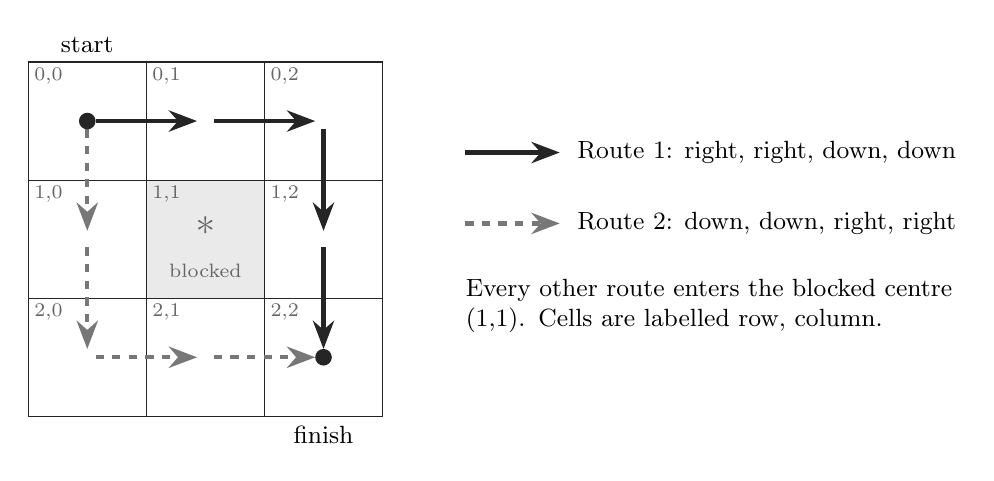
\begin{tikzpicture}[>=Stealth,every node/.style={font=\small},box/.style={draw=teal,rounded corners,minimum width=20mm,minimum height=8mm,fill=wash},arr/.style={->,thick,teal}]\draw[teal,fill=paper] (-0.75,-0.75) rectangle (0.75,0.75);\node[anchor=north west,inner sep=2pt,font=\scriptsize,text=quiet] at (-0.75,0.75) {0,0};\draw[teal,fill=paper] (0.75,-0.75) rectangle (2.25,0.75);\node[anchor=north west,inner sep=2pt,font=\scriptsize,text=quiet] at (0.75,0.75) {0,1};\draw[teal,fill=paper] (2.25,-0.75) rectangle (3.75,0.75);\node[anchor=north west,inner sep=2pt,font=\scriptsize,text=quiet] at (2.25,0.75) {0,2};\draw[teal,fill=paper] (-0.75,-2.25) rectangle (0.75,-0.75);\node[anchor=north west,inner sep=2pt,font=\scriptsize,text=quiet] at (-0.75,-0.75) {1,0};\draw[teal,fill=wash] (0.75,-2.25) rectangle (2.25,-0.75);\node[anchor=north west,inner sep=2pt,font=\scriptsize,text=quiet] at (0.75,-0.75) {1,1};\draw[teal,fill=paper] (2.25,-2.25) rectangle (3.75,-0.75);\node[anchor=north west,inner sep=2pt,font=\scriptsize,text=quiet] at (2.25,-0.75) {1,2};\draw[teal,fill=paper] (-0.75,-3.75) rectangle (0.75,-2.25);\node[anchor=north west,inner sep=2pt,font=\scriptsize,text=quiet] at (-0.75,-2.25) {2,0};\draw[teal,fill=paper] (0.75,-3.75) rectangle (2.25,-2.25);\node[anchor=north west,inner sep=2pt,font=\scriptsize,text=quiet] at (0.75,-2.25) {2,1};\draw[teal,fill=paper] (2.25,-3.75) rectangle (3.75,-2.25);\node[anchor=north west,inner sep=2pt,font=\scriptsize,text=quiet] at (2.25,-2.25) {2,2};\node[font=\Large,text=quiet,inner sep=0pt] at (1.5,-1.4) {*};\node[font=\scriptsize,text=quiet,inner sep=0pt] at (1.5,-1.9) {blocked};\node[anchor=south] at (0,0.75) {start};\node[anchor=north] at (3.0,-3.75) {finish};\draw[arr,line width=1.6pt,shorten >=3pt,shorten <=3pt] (0.0,0.0)--(1.5,0.0);\draw[arr,line width=1.6pt,shorten >=3pt,shorten <=3pt] (1.5,0.0)--(3.0,0.0);\draw[arr,line width=1.6pt,shorten >=3pt,shorten <=3pt] (3.0,0.0)--(3.0,-1.5);\draw[arr,line width=1.6pt,shorten >=3pt,shorten <=3pt] (3.0,-1.5)--(3.0,-3.0);\draw[arr,orange,dashed,line width=1.6pt,shorten >=3pt,shorten <=3pt] (0.0,0.0)--(0.0,-1.5);\draw[arr,orange,dashed,line width=1.6pt,shorten >=3pt,shorten <=3pt] (0.0,-1.5)--(0.0,-3.0);\draw[arr,orange,dashed,line width=1.6pt,shorten >=3pt,shorten <=3pt] (0.0,-3.0)--(1.5,-3.0);\draw[arr,orange,dashed,line width=1.6pt,shorten >=3pt,shorten <=3pt] (1.5,-3.0)--(3.0,-3.0);\fill[teal] (0.0,0.0) circle (3pt);\fill[teal] (3.0,-3.0) circle (3pt);\draw[arr,line width=1.6pt] (4.8,-0.4)--(6.0,-0.4);\node[anchor=west] at (6.1,-0.4) {Route 1: right, right, down, down};\draw[arr,orange,dashed,line width=1.6pt] (4.8,-1.3)--(6.0,-1.3);\node[anchor=west] at (6.1,-1.3) {Route 2: down, down, right, right};\node[anchor=north west,text width=62mm,inner sep=0pt] at (4.8,-2.0) {Every other route enters the blocked centre (1,1). Cells are labelled row, column.};\end{tikzpicture}\end{center}\end{minipage}
\par\bigskip\begin{minipage}{\textwidth}\textbf{L2-10 / A grid cell receives two counts}\par\par\medskip \begingroup\small\setlength{\tabcolsep}{4pt}\renewcommand{\arraystretch}{1.35}\begin{tabularx}{\linewidth}{>{\raggedright\arraybackslash}X>{\raggedright\arraybackslash}X>{\raggedright\arraybackslash}X>{\raggedright\arraybackslash}X}\toprule\textbf{Row / column} & \textbf{0} & \textbf{1} & \textbf{2}\\\midrule
0 & 1 & 1 & 1\\
1 & 1 & 0 & 1\\
2 & 1 & 1 & 2\\
\bottomrule\end{tabularx}\endgroup\par\medskip \end{minipage}
\par\bigskip\begin{minipage}{\textwidth}\textbf{L2-13 / Your turn: test the boundaries}\par\par\medskip \begingroup\small\setlength{\tabcolsep}{4pt}\renewcommand{\arraystretch}{1.35}\begin{tabularx}{\linewidth}{>{\raggedright\arraybackslash}X>{\raggedright\arraybackslash}X>{\raggedright\arraybackslash}X}\toprule\textbf{Test grid} & \textbf{Your prediction} & \textbf{Program output}\\\midrule
{}['.']  (one open cell) & 1 & 1\\
{}['*']  (one blocked cell) & 0 & 0\\
{}['..', '..']  (open 2 by 2) & 2 & 2\\
{}['...', '.*.', '...']  (centre blocked) & 2 & 2\\
\bottomrule\end{tabularx}\endgroup\par\medskip \end{minipage}
\topicflow{CODE ANSWERS}{Complete code}
Every function used in class, in question order. Line numbers are the same as in the tutor book.\par\medskip
\Needspace{12\baselineskip}
{\color{teal}\textbf{L2-04}}\quad\textbf{\texttt{dice\_slow}}\label{L2-code-dice_slow}\par
\begin{lstlisting}[style=numbered]
def dice_slow(n):
    if n == 0:
        return 1
    return sum(dice_slow(n - face) for face in range(1, min(6, n) + 1))
\end{lstlisting}
\textbf{Recursion depth.} Python stops recursion at about 1,000 nested calls by default, so this recursive version is for small inputs and the small and edge test files only. Use the iterative version for the medium and large files.

\par\bigskip
\Needspace{18\baselineskip}
{\color{teal}\textbf{L2-04}}\quad\textbf{\texttt{dice\_cached}}\label{L2-code-dice_cached}\par
\begin{lstlisting}[style=numbered]
MOD = 1_000_000_007

def dice_cached(n):
    cache = {0: 1}
    def count(total):
        if total not in cache:
            cache[total] = sum(count(total - face)
                for face in range(1, min(6, total) + 1)) % MOD
        return cache[total]
    return count(n)
\end{lstlisting}
\textbf{Recursion depth.} Python stops recursion at about 1,000 nested calls by default, so this recursive version is for small inputs and the small and edge test files only. Use the iterative version for the medium and large files.

\par\bigskip
\Needspace{20\baselineskip}
{\color{teal}\textbf{L2-05}}\quad\textbf{\texttt{dice\_table}}\label{L2-code-dice_table}\par
\begin{lstlisting}[style=numbered]
MOD = 1_000_000_007

def dice_table(n):
    ways = [0] * (n + 1)
    ways[0] = 1
    for total in range(1, n + 1):
        for face in range(1, 7):
            if total >= face:
                ways[total] += ways[total - face]
        ways[total] %= MOD
    return ways[n]
\end{lstlisting}

\begin{lstlisting}
print(dice_table(7))
\end{lstlisting}
\textbf{Expected output:} 63
\par\bigskip
\Needspace{20\baselineskip}
{\color{teal}\textbf{L2-07}}\quad\textbf{\texttt{dice\_123}}\label{L2-code-dice_123}\par
\begin{lstlisting}[style=numbered]
MOD = 1_000_000_007

def dice_123(n):
    ways = [0] * (n + 1)
    ways[0] = 1
    for total in range(1, n + 1):
        for face in (1, 2, 3):
            if total >= face:
                ways[total] += ways[total - face]
        ways[total] %= MOD
    return ways[n]
\end{lstlisting}

\begin{lstlisting}
print([dice_123(n) for n in range(6)])
\end{lstlisting}
\textbf{Expected output:} [1, 1, 2, 4, 7, 13]
\par\bigskip
\Needspace{14\baselineskip}
{\color{teal}\textbf{L2-08}}\quad\textbf{\texttt{dice\_ring}}\label{L2-code-dice_ring}\par
\begin{lstlisting}[style=numbered]
MOD = 1_000_000_007

def dice_ring(n):
    recent = [0] * 6
    recent[0] = 1
    for total in range(1, n + 1):
        answer = sum(recent) % MOD
        recent[total % 6] = answer
    return recent[n % 6]
\end{lstlisting}
\par\bigskip
\Needspace{17\baselineskip}
{\color{teal}\textbf{L2-08}}\quad\textbf{\texttt{dice\_window}}\label{L2-code-dice_window}\par
\begin{lstlisting}[style=numbered]
MOD = 1_000_000_007

def dice_window(n):
    recent = [0] * 6
    recent[0] = 1
    window = 1
    for total in range(1, n + 1):
        slot = total % 6
        oldest = recent[slot]
        recent[slot] = window
        window = (window - oldest + recent[slot]) % MOD
    return recent[n % 6]
\end{lstlisting}
\par\bigskip
\Needspace{17\baselineskip}
{\color{teal}\textbf{L2-11}}\quad\textbf{\texttt{grid\_slow}}\label{L2-code-grid_slow}\par
\begin{lstlisting}[style=numbered]
def grid_slow(rows):
    n = len(rows)
    def count(r, c):
        if r < 0 or c < 0 or rows[r][c] == '*':
            return 0
        if r == 0 and c == 0:
            return 1
        return count(r - 1, c) + count(r, c - 1)
    return count(n - 1, n - 1)
\end{lstlisting}
\textbf{Recursion depth.} Python stops recursion at about 1,000 nested calls by default, so this recursive version is for small inputs and the small and edge test files only. Use the iterative version for the medium and large files.

\par\bigskip
\Needspace{22\baselineskip}
{\color{teal}\textbf{L2-11}}\quad\textbf{\texttt{grid\_cached}}\label{L2-code-grid_cached}\par
\begin{lstlisting}[style=numbered]
from functools import lru_cache

MOD = 1_000_000_007

def grid_cached(rows):
    n = len(rows)
    @lru_cache(None)
    def count(r, c):
        if r < 0 or c < 0 or rows[r][c] == '*':
            return 0
        if r == 0 and c == 0:
            return 1
        return (count(r - 1, c) + count(r, c - 1)) % MOD
    return count(n - 1, n - 1)
\end{lstlisting}
\textbf{Recursion depth.} Python stops recursion at about 1,000 nested calls by default, so this recursive version is for small inputs and the small and edge test files only. Use the iterative version for the medium and large files.

\par\bigskip
\Needspace{25\baselineskip}
{\color{teal}\textbf{L2-12}}\quad\textbf{\texttt{grid\_table}}\label{L2-code-grid_table}\par
\begin{lstlisting}[style=numbered]
MOD = 1_000_000_007

def grid_table(rows):
    n = len(rows)
    paths = [[0] * n for _ in range(n)]
    for r in range(n):
        for c in range(n):
            if rows[r][c] == '*':
                continue
            if r == 0 and c == 0:
                paths[r][c] = 1
            else:
                above = paths[r - 1][c] if r > 0 else 0
                left = paths[r][c - 1] if c > 0 else 0
                paths[r][c] = (above + left) % MOD
    return paths[-1][-1]
\end{lstlisting}

\begin{lstlisting}
print(grid_table(['...', '.*.', '...']))
\end{lstlisting}
\textbf{Expected output:} 2
\par\bigskip
\topicflow{EXERCISE CHECKS}{Expected notebook results}
\Needspace{8\baselineskip}\textbf{L2-07 / dice\_123}\par
Use the complete \texttt{dice\_123} solution on page~\pageref{L2-code-dice_123}. The function name and parameters are the same in the notebook.

\begin{lstlisting}
dice_123(0)  # expected: 1
dice_123(4)  # expected: 7
dice_123(5)  # expected: 13
\end{lstlisting}
\Needspace{8\baselineskip}\textbf{L2-13 / grid\_table}\par
Use the complete \texttt{grid\_table} solution on page~\pageref{L2-code-grid_table}. The function name and parameters are the same in the notebook.

\begin{lstlisting}
grid_table(['.'])                  # expected: 1
grid_table(['*'])                  # expected: 0
grid_table(['..', '..'])           # expected: 2
grid_table(['...', '.*.', '...'])  # expected: 2
\end{lstlisting}
\clearpage\renewcommand{\lessonnumber}{3}\renewcommand{\lessonheading}{Lesson 3 · Mortal Kombat Tower and Array Description}\phantomsection\label{lesson-3}\pdfbookmark[-1]{Lesson 3: Mortal Kombat Tower and Array Description}{lesson-3-bookmark}
\noindent\makebox[\linewidth][l]{\begin{minipage}{176mm}{\heavy\fontsize{23}{28}\selectfont\raggedright Lesson 3\par}\vspace{2mm}{\heavy\fontsize{19}{24}\selectfont\raggedright Mortal Kombat Tower and Array Description\par}\end{minipage}}\par\vspace{5mm}
\href{https://colab.research.google.com/github/fifteen02/julians-pathfinder/blob/main/Lesson\%203/lesson.ipynb}{\underline{Open this lesson in Google Colab}}\par
\topicflow{BEFORE CLASS}{The lesson route}
\par\noindent\colorbox{wash}{\parbox{\dimexpr\linewidth-2\fboxsep\relax}{\vspace{3pt}{\color{quiet}\heavy\fontsize{8.5}{10}\selectfont MAIN IDEA: SAY THIS AT THE START}\par\smallskip{\heavy\fontsize{15}{18}\selectfont Remember the missing detail.}\par\smallskip If the position alone cannot tell what happens next, also remember the detail that does: whose turn it is, or the previous value.\par\medskip\textbf{By the end of the lesson you will be able to}\begin{itemize}\item explain why the boss position alone is not enough in Tower;\item fill friend[i] and you[i] from the last boss back to the first;\item count array fillings with table[i][v], keeping the previous value.\end{itemize}\vspace{3pt}}}\par

The target is understanding, not finishing every page. Use the question IDs to move between slides, worksheet and notebook.

\begingroup\small\setlength{\tabcolsep}{4pt}\renewcommand{\arraystretch}{1.35}\begin{tabularx}{\linewidth}{>{\raggedright\arraybackslash}p{18mm}>{\raggedright\arraybackslash}X>{\raggedright\arraybackslash}p{38mm}}\toprule\textbf{Minutes} & \textbf{Activity} & \textbf{Question IDs}\\\midrule
0-10 & When one index is not enough & L3-01\\
10-25 & Act out the Tower rules & L3-02 to L3-03\\
25-45 & Recursive state and cached solution & L3-04\\
45-60 & Backward table and student trace & L3-05 to L3-06\\
60-65 & Break & \\
65-80 & Enumerate missing array values & L3-07 to L3-08\\
80-100 & Cached recursion and full table & L3-09 to L3-10\\
100-115 & Rolling rows and student exercise & L3-11 to L3-12\\
115-120 & Exit: identify the missing detail & L3-13\\
\bottomrule\end{tabularx}\endgroup

\labeltext{Pacing and preparation}
Ask students to predict before running code. Allow a quiet individual attempt before asking for a volunteer. If an answer is wrong, trace the first state where it differs. Keep the final ten minutes for explanation and questions. Move an unfinished implementation to the next session rather than shortening the reasoning.

Students need Python functions, lists, loops, indexing, comparisons and basic arithmetic. Introduce new syntax beside the program that uses it. Use small inputs for uncached recursion; the notebook never starts an enormous recursive run. Python stops recursion at about 1,000 nested calls by default, so every recursive version in this lesson, cached or not, is for small inputs and the small and edge test files only. The medium and large files are for the iterative versions.

Open lesson.ipynb in Jupyter or upload it to Google Colab, choose a Python 3 runtime, and run the setup cell first. Shift+Enter runs a cell. Restart and run from the top if names or data become stale. The notebook needs only Python standard-library features and no local files.
\topic{KEEP BESIDE YOUR WORK}{The route and the rules}
\textbf{Our route}\par Ask what extra information changes the available choices. Tower needs the next player as well as the boss position. Array Description needs the neighbouring value as well as the position. Work a small case, describe the stored answer, then write recursion and a table.\par\medskip
\textbf{Tower rules · L3-01 to L3-06}\par Bosses are listed in order: 0 means easy and 1 means hard. Your friend starts. On each turn, the player must defeat the next one or two remaining bosses, then the other player moves. Your friend pays one point for each hard boss they defeat; you pay nothing. Both players cooperate to minimise the friend's total payment.\par\medskip
\textbf{Tower names}\par \texttt{n} is the number of bosses. Position \texttt{i} identifies the next boss to defeat. \texttt{friend\_turn} is True when your friend plays next and False when you play next. Position n means no bosses remain; it is just beyond the last valid list index.\par\medskip
\textbf{Array rules · L3-07 to L3-13}\par Fill every missing entry with an integer from 1 to m. A 0 in the input marks a missing entry; 0 is not allowed in the completed array. Keep fixed entries unchanged. Two neighbouring values may differ by at most 1. Count all valid completed arrays, returning the count modulo 1,000,000,007.\par\medskip
\textbf{Array names}\par \texttt{n} is the number of entries and \texttt{m} is the largest allowed value. \texttt{i} is a position, starting at 0; \texttt{v} is a possible value placed there. A prefix through position i means the entries from position 0 up to and including position i. For example, the prefix through position 1 of [2, 3, 2] is [2, 3].\par\medskip
\topicflow{IN CLASS}{Questions, answers and prompts}
\markboth{Tower: remember whose turn comes next}{}{\color{quiet}\heavy\fontsize{10}{13}\selectfont TOWER: REMEMBER WHOSE TURN COMES NEXT}\par\medskip
\noindent\begin{minipage}{\textwidth}
{\color{teal}\textbf{L3-01}}\quad \textbf{When one index is not enough}\par\smallskip
\textbf{Ask.} One hard boss remains. If your friend takes the next turn, defeating it costs one point. If you take the next turn, it costs no points. Can the boss position alone identify the minimum remaining payment? What other detail must the question include?\par\smallskip
\textbf{Answer.} No. The same remaining bosses can cost different amounts depending on whose turn comes next. We must record both the position and the player who moves next.\par\smallskip
\textbf{Prompt if stuck.} Compare the same final hard boss on each player's turn.\par\smallskip
\textbf{Watch for.} A cheaper history cannot replace another history if it leaves a different player to move.
\end{minipage}\par\medskip{\color{lightink}\hrule height .4pt}\medskip

\noindent\begin{minipage}{\textwidth}
{\color{teal}\textbf{L3-02}}\quad \textbf{Tower rules at the board}\par\smallskip
\textbf{Ask.} Bosses are [1, 0, 1, 1]: 1 is hard and 0 is easy. Your friend starts. Players alternate turns, each defeating the next one or two bosses. Only your friend pays, one point per hard boss they defeat. Both players cooperate. Find a schedule with the smallest total payment.\par\smallskip
\textbf{Answer.} The friend beats bosses 0 and 1, paying 1. You beat bosses 2 and 3, paying 0. Total: 1. At least one point is unavoidable because the friend must face the first hard boss.\par\smallskip
\textbf{Prompt if stuck.} The first boss forces a lower bound of one point.\par\smallskip
\textbf{Watch for.} The friend cannot choose to take zero bosses or let you start.
\end{minipage}\par\medskip{\color{lightink}\hrule height .4pt}\medskip

\noindent\begin{minipage}{\textwidth}
{\color{teal}\textbf{L3-03}}\quad \textbf{Name the remaining question}\par\smallskip
\textbf{Ask.} Let n be the number of bosses and i the next boss position, starting at 0. friend\_turn is True for your friend and False for you. Define cost(i, friend\_turn) in a sentence: does it include earlier payments? What should it return when i = n?\par\smallskip
\textbf{Answer.} cost(i, friend\_turn) is the smallest additional payment for all bosses from position i onwards, with that player moving next. It excludes payments already made. At i = n, no bosses remain, so both turn states return 0. The whole-game question is cost(0, True).\par\smallskip
\textbf{Prompt if stuck.} Complete the sentence: the least additional cost starting at...\par\smallskip
\textbf{Watch for.} Confusing remaining cost with cost already paid reverses the interpretation of the table.
\end{minipage}\par\medskip{\color{lightink}\hrule height .4pt}\medskip

\noindent\begin{minipage}{\textwidth}
{\color{teal}\textbf{L3-04}}\quad \textbf{Compare a session and its continuation}\par\smallskip
\textbf{Ask.} Write tower\_cached(bosses) using cached recursion. From position i, write the two legal Tower choices. How does payment depend on the player? Use these choices in your function.\par\smallskip
\par\smallskip{\small\textbf{Students start with:}}\par\smallskip\noindent\colorbox{codepaper}{\parbox{\dimexpr\linewidth-2\fboxsep\relax}{\small\ttfamily\raggedright def tower\_cached(bosses):\\\hspace*{2.4em}def cost(i, friend\_turn):\\\hspace*{4.8em}return None  \# Your helper goes here.\\\hspace*{2.4em}return cost(0, True)}}\par
{\small\textbf{What each function returns.}\par tower\_cached(bosses): the minimum total points paid by your friend, who starts.\par cost(i, friend\_turn): the minimum further points your friend must pay from boss i, with the indicated player next.\par }
{\small\textbf{Hints to give, one at a time.}}\begin{itemize}\item What is the remaining cost when no bosses remain?\item On one turn, how many bosses can the player take, and who pays for them?\item After the turn, who plays next, and from which position?\end{itemize}
\textbf{Answer.} Take one boss or, if available, two. The friend pays the sum of those boss values; you pay zero. Add the continuation at i + take with the other player moving next. Choose the smaller total.\par\smallskip
\textbf{Prompt if stuck.} After every session, switch the turn exactly once.\par\smallskip
\textbf{Watch for.} Hard bosses are charged only when friend\_turn is True.\par\smallskip Full code: \texttt{tower\_cached} (page~\pageref{L3-code-tower_cached}).
\end{minipage}\par\medskip{\color{lightink}\hrule height .4pt}\medskip

\noindent\begin{minipage}{\textwidth}
{\color{teal}\textbf{L3-05}}\quad \textbf{A table filled from the end}\par\smallskip
\textbf{Ask.} Let friend[i] and you[i] be the least remaining cost when that player moves next at boss i. Fill both lists for [1, 0, 1, 1]. In which direction must the loop run?\par\smallskip
\textbf{Answer.} friend = [1, 0, 1, 1, 0] and you = [0, 1, 0, 0, 0]. Position 4 is preset to 0; the loop fills positions 3 down to 0 because each state reads positions i + 1 or i + 2. The required answer is friend[0] = 1.\par\smallskip
\textbf{Prompt if stuck.} Start with the row where no bosses remain.\par\smallskip
\textbf{Watch for.} Returning min(friend[0], you[0]) incorrectly lets you take the first turn.\par\smallskip Full code: \texttt{tower\_table} (page~\pageref{L3-code-tower_table}).
\end{minipage}\par\medskip{\color{lightink}\hrule height .4pt}\medskip

\noindent\begin{minipage}{\textwidth}
{\color{teal}\textbf{L3-06}}\quad \textbf{Your turn: Tower boundaries}\par\smallskip
\textbf{Ask.} Write tower\_table(bosses) using loops to fill the two lists from L3-05. Test bosses [0], [1] and [1, 1, 1]. Give a schedule for the third case. Explain why the two-boss option needs a bounds check.\par\smallskip
\par\smallskip{\small\textbf{Students start with:}}\par\smallskip\noindent\colorbox{codepaper}{\parbox{\dimexpr\linewidth-2\fboxsep\relax}{\small\ttfamily\raggedright def tower\_table(bosses):\\\hspace*{2.4em}return None  \# Replace with your answer.}}\par
{\small\textbf{What each function returns.}\par tower\_table(bosses): the minimum total points paid by your friend, who starts.\par }
{\small\textbf{Hints to give, one at a time.}}\begin{itemize}\item Which positions are filled before the loop?\item In which direction must i move so that positions i + 1 and i + 2 are ready?\item Which entry is the answer, given that your friend starts?\end{itemize}
\textbf{Answer.} The answers are 0, 1 and 1. For three hard bosses, the friend takes one and you take two. At the final boss, taking two would go past the end, so only the one-boss option is legal.\par\smallskip
\textbf{Prompt if stuck.} The friend pays only for bosses taken during the friend's sessions.\par\smallskip
\textbf{Watch for.} Accessing bosses[i + 1] at the final boss is an index error.
\end{minipage}\par\medskip{\color{lightink}\hrule height .4pt}\medskip

\Needspace{14\baselineskip}\markboth{Arrays: remember the neighbouring value}{}{\color{quiet}\heavy\fontsize{10}{13}\selectfont ARRAYS: REMEMBER THE NEIGHBOURING VALUE}\par\medskip
\noindent\begin{minipage}{\textwidth}
{\color{teal}\textbf{L3-07}}\quad \textbf{Array Description: fill the gaps}\par\smallskip
\textbf{Ask.} Values must be from 1 to 3 and neighbouring values may differ by at most 1. In [2, 0, 0, 1], zero means missing. List all valid completed arrays.\par\smallskip
\textbf{Answer.} The five arrays are [2,1,1,1], [2,1,2,1], [2,2,1,1], [2,2,2,1] and [2,3,2,1]. Zero is a placeholder, not an allowed final value.\par\smallskip
\textbf{Prompt if stuck.} Choose the second entry, then test which third entries can also touch the final 1.\par\smallskip
\textbf{Watch for.} Treating a missing zero as an actual value changes the problem.
\end{minipage}\par\medskip{\color{lightink}\hrule height .4pt}\medskip

\noindent\begin{minipage}{\textwidth}
{\color{teal}\textbf{L3-08}}\quad \textbf{Position and last value}\par\smallskip
\textbf{Ask.} Let table[i][v] count valid fillings of positions 0 through i whose value at position i is v. Position i and value v have different jobs. If v = 2, which previous values may contribute? If the input fixes position i to 1, which columns must contain 0?\par\smallskip
\textbf{Answer.} table[i][v] counts valid fillings through position i whose final value is v. For v = 2, previous values 1, 2 and 3 may contribute. If position i is fixed to 1, counts for v = 2 and v = 3 are zero.\par\smallskip
\textbf{Prompt if stuck.} Write the column heading as final value, not position.\par\smallskip
\textbf{Watch for.} Keeping only a total across all final values loses the neighbour information.
\end{minipage}\par\medskip{\color{lightink}\hrule height .4pt}\medskip

\noindent\begin{minipage}{\textwidth}
{\color{teal}\textbf{L3-09}}\quad \textbf{Array recursion remembers the previous value}\par\smallskip
\textbf{Ask.} Write array\_cached(values, m) using cached recursion for Array Description. What does the helper need besides the next position to fill?\par\smallskip
\par\smallskip{\small\textbf{Students start with:}}\par\smallskip\noindent\colorbox{codepaper}{\parbox{\dimexpr\linewidth-2\fboxsep\relax}{\small\ttfamily\raggedright def array\_cached(values, m):\\\hspace*{2.4em}def count(i, previous):\\\hspace*{4.8em}return None  \# Your helper goes here.\\\hspace*{2.4em}return count(0, 0)}}\par
{\small\textbf{What each function returns.}\par array\_cached(values, m): the number of valid completed arrays, modulo 1,000,000,007.\par count(i, previous): the number of valid completions from position i with the given previous value, modulo 1,000,000,007.\par }
{\small\textbf{Hints to give, one at a time.}}\begin{itemize}\item What does count return when every position has been filled?\item Which values may position i take if the input fixes it?\item How does the previous value restrict the next value?\end{itemize}
\textbf{Answer.} It needs the previous value. Try every allowed value for the current position, check the neighbour rule, then recurse on the next position with that new value. Reaching the end contributes one completed array.\par\smallskip
\textbf{Prompt if stuck.} When a position is fixed, reject every candidate except that value.\par\smallskip
\textbf{Watch for.} The sentinel previous = 0 is not a permitted value in a completed array.\par\smallskip Full code: \texttt{array\_cached} (page~\pageref{L3-code-array_cached}).
\end{minipage}\par\medskip{\color{lightink}\hrule height .4pt}\medskip

\noindent\begin{minipage}{\textwidth}
{\color{teal}\textbf{L3-10}}\quad \textbf{The full array-count table}\par\smallskip
\textbf{Ask.} For input [2, 0, 0, 1], allow values 1 to 3. Fill table[i][v]: the number of valid fillings through position i ending in value v. The first row is supplied. Explain one entry in the next row, then complete the table. Which final-row entries contribute to the total?\par\smallskip
\textbf{Answer.} The rows are [0,1,0], [1,1,1], [2,3,2], [5,0,0]. For example, table[1][1] is 1: the only permitted prefix is [2,1]. Sum the final row to get 5. Only its column for value 1 is nonzero because the last input entry is fixed to 1.\par\smallskip
\textbf{Prompt if stuck.} Each new cell adds at most three cells from the previous row.\par\smallskip
\textbf{Watch for.} Setting every first-row column to one ignores a fixed first entry.\par\smallskip Full code: \texttt{array\_full} (page~\pageref{L3-code-array_full}).
\end{minipage}\par\medskip{\color{lightink}\hrule height .4pt}\medskip

\noindent\begin{minipage}{\textwidth}
{\color{teal}\textbf{L3-11}}\quad \textbf{Keep the previous row intact}\par\smallskip
\textbf{Ask.} Let n be the array length and m the largest allowed value. before[v] holds the count ending in v at the previous position; now[v] holds it at the current position. Why do two rows suffice? Why must we finish now before assigning before = now?\par\smallskip
\textbf{Answer.} Each new row reads only the previous row, so two rows suffice. With previous counts [1,1,1], the new count for value 1 is 1 + 1 = 2. If we overwrite the first previous count with 2, the calculation for value 2 wrongly reads 2 + 1 + 1 = 4 instead of 3. Keep the previous row intact.\par\smallskip
\textbf{Prompt if stuck.} Ask whether column v + 1 still belongs to the previous position when you read it.\par\smallskip
\textbf{Watch for.} Moving before = now inside the loop over values changes the row too early.\par\smallskip Full code: \texttt{array\_rolling} (page~\pageref{L3-code-array_rolling}).
\end{minipage}\par\medskip{\color{lightink}\hrule height .4pt}\medskip

\noindent\begin{minipage}{\textwidth}
{\color{teal}\textbf{L3-12}}\quad \textbf{Your turn: an unknown prefix}\par\smallskip
\textbf{Ask.} Write array\_rolling(values, m) using a loop and two rows. First complete [0, 0, 3] using values 1 to 3, with neighbouring values differing by at most 1: fill the table and list all valid arrays. Then write your code and test both [0, 0, 3] and [1, 3] with m = 3. Explain each result.\par\smallskip
\par\smallskip{\small\textbf{Students start with:}}\par\smallskip\noindent\colorbox{codepaper}{\parbox{\dimexpr\linewidth-2\fboxsep\relax}{\small\ttfamily\raggedright def array\_rolling(values, m):\\\hspace*{2.4em}return None  \# Replace with your answer.}}\par
{\small\textbf{What each function returns.}\par array\_rolling(values, m): the number of valid completed arrays, modulo 1,000,000,007.\par }
{\small\textbf{Hints to give, one at a time.}}\begin{itemize}\item What does the first row look like, when there is no previous value?\item Which entries of the previous row can lead to value v?\item Why must the new row be built separately from the old row?\end{itemize}
\textbf{Answer.} The rows are [1,1,1], [2,3,2], [0,0,5]. Valid arrays: [1,2,3], [2,2,3], [3,2,3], [2,3,3], [3,3,3]. The fixed array [1,3] has zero valid fillings.\par\smallskip
\textbf{Prompt if stuck.} The final 3 can follow only 2 or 3.\par\smallskip
\textbf{Watch for.} Returning only the final column works for this example but not when the last entry is unknown.
\end{minipage}\par\medskip{\color{lightink}\hrule height .4pt}\medskip

\noindent\begin{minipage}{\textwidth}
{\color{teal}\textbf{L3-13}}\quad \textbf{What information changes the future?}\par\smallskip
\textbf{Ask.} Why does Tower need the next player, while Array Description needs the previous value? What details can we forget in each problem?\par\smallskip
\textbf{Answer.} The next player changes Tower payments. The previous value changes legal array neighbours. Once these details and the position are known, the rest of the earlier history does not change the remaining choices.\par\smallskip
\textbf{Prompt if stuck.} Construct two histories at the same position with different next possibilities.\par\smallskip
\textbf{Watch for.} More dimensions are justified by information, not by a desire to use a larger table.
\end{minipage}\par\medskip{\color{lightink}\hrule height .4pt}\medskip

\topicflow{TRACE ANSWERS}{Completed diagrams and tables}
\par\bigskip\begin{minipage}{\textwidth}\textbf{L3-05 / A table filled from the end}\par\par\medskip \begingroup\small\setlength{\tabcolsep}{4pt}\renewcommand{\arraystretch}{1.35}\begin{tabularx}{\linewidth}{>{\raggedright\arraybackslash}X>{\raggedright\arraybackslash}X>{\raggedright\arraybackslash}X>{\raggedright\arraybackslash}X>{\raggedright\arraybackslash}X>{\raggedright\arraybackslash}X}\toprule\textbf{Next boss i} & \textbf{0} & \textbf{1} & \textbf{2} & \textbf{3} & \textbf{4}\\\midrule
friend[i] & 1 & 0 & 1 & 1 & 0\\
you[i] & 0 & 1 & 0 & 0 & 0\\
\bottomrule\end{tabularx}\endgroup\par\medskip \end{minipage}
\par\bigskip\begin{minipage}{\textwidth}\textbf{L3-10 / The full array-count table}\par\par\medskip \begingroup\small\setlength{\tabcolsep}{4pt}\renewcommand{\arraystretch}{1.35}\begin{tabularx}{\linewidth}{>{\raggedright\arraybackslash}X>{\raggedright\arraybackslash}X>{\raggedright\arraybackslash}X>{\raggedright\arraybackslash}X>{\raggedright\arraybackslash}X}\toprule\textbf{Position} & \textbf{Given} & \textbf{v = 1} & \textbf{v = 2} & \textbf{v = 3}\\\midrule
0 & 2 & 0 & 1 & 0\\
1 & 0 & 1 & 1 & 1\\
2 & 0 & 2 & 3 & 2\\
3 & 1 & 5 & 0 & 0\\
\bottomrule\end{tabularx}\endgroup\par\medskip \end{minipage}
\par\bigskip\begin{minipage}{\textwidth}\textbf{L3-12 / Your turn: an unknown prefix}\par\par\medskip \begingroup\small\setlength{\tabcolsep}{4pt}\renewcommand{\arraystretch}{1.35}\begin{tabularx}{\linewidth}{>{\raggedright\arraybackslash}X>{\raggedright\arraybackslash}X>{\raggedright\arraybackslash}X>{\raggedright\arraybackslash}X>{\raggedright\arraybackslash}X}\toprule\textbf{Position} & \textbf{Given} & \textbf{v = 1} & \textbf{v = 2} & \textbf{v = 3}\\\midrule
0 & 0 & 1 & 1 & 1\\
1 & 0 & 2 & 3 & 2\\
2 & 3 & 0 & 0 & 5\\
\bottomrule\end{tabularx}\endgroup\par\medskip \end{minipage}
\topicflow{CODE ANSWERS}{Complete code}
Every function used in class, in question order. Line numbers are the same as in the tutor book.\par\medskip
\Needspace{27\baselineskip}
{\color{teal}\textbf{L3-04}}\quad\textbf{\texttt{tower\_cached}}\label{L3-code-tower_cached}\par
\begin{lstlisting}[style=numbered]
from functools import lru_cache

def tower_cached(bosses):
    n = len(bosses)
    @lru_cache(None)
    def cost(i, friend_turn):
        if i == n:
            return 0
        answer = float('inf')
        for take in (1, 2):
            if i + take <= n:
                pay = sum(bosses[i:i + take]) if friend_turn else 0
                answer = min(answer, pay + cost(i + take, not friend_turn))
        return answer
    return cost(0, True)
\end{lstlisting}
\textbf{Recursion depth.} Python stops recursion at about 1,000 nested calls by default, so this recursive version is for small inputs and the small and edge test files only. Use the iterative version for the medium and large files.


\begin{lstlisting}
print(tower_cached([1, 0, 1, 1]))
\end{lstlisting}
\textbf{Expected output:} 1
\par\bigskip
\Needspace{21\baselineskip}
{\color{teal}\textbf{L3-05}}\quad\textbf{\texttt{tower\_table}}\label{L3-code-tower_table}\par
\begin{lstlisting}[style=numbered]
def tower_table(bosses):
    n = len(bosses)
    friend = [0] * (n + 1)
    you = [0] * (n + 1)
    for i in range(n - 1, -1, -1):
        friend[i] = bosses[i] + you[i + 1]
        you[i] = friend[i + 1]
        if i + 1 < n:
            pay = bosses[i] + bosses[i + 1]
            friend[i] = min(friend[i], pay + you[i + 2])
            you[i] = min(you[i], friend[i + 2])
    return friend[0]
\end{lstlisting}

\begin{lstlisting}
print(tower_table([1, 0, 1, 1]))
\end{lstlisting}
\textbf{Expected output:} 1
\par\bigskip
\Needspace{29\baselineskip}
{\color{teal}\textbf{L3-09}}\quad\textbf{\texttt{array\_cached}}\label{L3-code-array_cached}\par
\begin{lstlisting}[style=numbered]
from functools import lru_cache

MOD = 1_000_000_007

def array_cached(values, m):
    @lru_cache(None)
    def count(i, previous):
        if i == len(values):
            return 1
        answer = 0
        for value in range(1, m + 1):
            if values[i] != 0 and values[i] != value:
                continue
            if i == 0 or abs(value - previous) <= 1:
                answer += count(i + 1, value)
        return answer % MOD
    return count(0, 0)
\end{lstlisting}
\textbf{Recursion depth.} Python stops recursion at about 1,000 nested calls by default, so this recursive version is for small inputs and the small and edge test files only. Use the iterative version for the medium and large files.


\begin{lstlisting}
print(array_cached([2, 0, 0, 1], 3))
\end{lstlisting}
\textbf{Expected output:} 5
\par\bigskip
\Needspace{22\baselineskip}
{\color{teal}\textbf{L3-10}}\quad\textbf{\texttt{array\_full}}\label{L3-code-array_full}\par
\begin{lstlisting}[style=numbered]
MOD = 1_000_000_007

def array_full(values, m):
    table = [[0] * (m + 2) for _ in values]
    for value in range(1, m + 1):
        if values[0] in (0, value):
            table[0][value] = 1
    for i in range(1, len(values)):
        for value in range(1, m + 1):
            if values[i] in (0, value):
                table[i][value] = (table[i - 1][value - 1] + table[i - 1][value]
                                   + table[i - 1][value + 1]) % MOD
    return sum(table[-1]) % MOD
\end{lstlisting}

\begin{lstlisting}
print(array_full([2, 0, 0, 1], 3))
\end{lstlisting}
\textbf{Expected output:} 5
\par\bigskip
\Needspace{24\baselineskip}
{\color{teal}\textbf{L3-11}}\quad\textbf{\texttt{array\_rolling}}\label{L3-code-array_rolling}\par
\begin{lstlisting}[style=numbered]
MOD = 1_000_000_007

def array_rolling(values, m):
    before = [0] * (m + 2)
    for value in range(1, m + 1):
        if values[0] in (0, value):
            before[value] = 1
    for i in range(1, len(values)):
        now = [0] * (m + 2)
        for value in range(1, m + 1):
            if values[i] in (0, value):
                now[value] = (before[value - 1] + before[value]
                              + before[value + 1]) % MOD
        before = now
    return sum(before) % MOD
\end{lstlisting}

\begin{lstlisting}
print(array_rolling([2, 0, 0, 1], 3))
\end{lstlisting}
\textbf{Expected output:} 5
\par\bigskip
\topicflow{EXERCISE CHECKS}{Expected notebook results}
\Needspace{8\baselineskip}\textbf{L3-06 / tower\_table}\par
Use the complete \texttt{tower\_table} solution on page~\pageref{L3-code-tower_table}. The function name and parameters are the same in the notebook.

\begin{lstlisting}
tower_table([0])        # expected: 0
tower_table([1])        # expected: 1
tower_table([1,1,1])    # expected: 1
tower_table([1,0,1,1])  # expected: 1
\end{lstlisting}
\Needspace{8\baselineskip}\textbf{L3-12 / array\_rolling}\par
Use the complete \texttt{array\_rolling} solution on page~\pageref{L3-code-array_rolling}. The function name and parameters are the same in the notebook.

\begin{lstlisting}
array_rolling([0,0,3], 3)  # expected: 5
array_rolling([1,3], 3)    # expected: 0
array_rolling([0], 3)      # expected: 3
\end{lstlisting}
\clearpage\renewcommand{\lessonnumber}{4}\renewcommand{\lessonheading}{Lesson 4 · Fruit Feast}\phantomsection\label{lesson-4}\pdfbookmark[-1]{Lesson 4: Fruit Feast}{lesson-4-bookmark}
\noindent\makebox[\linewidth][l]{\begin{minipage}{176mm}{\heavy\fontsize{23}{28}\selectfont\raggedright Lesson 4\par}\vspace{2mm}{\heavy\fontsize{19}{24}\selectfont\raggedright Fruit Feast\par}\end{minipage}}\par\vspace{5mm}
\href{https://colab.research.google.com/github/fifteen02/julians-pathfinder/blob/main/Lesson\%204/lesson.ipynb}{\underline{Open this lesson in Google Colab}}\par
\topicflow{BEFORE CLASS}{The lesson route}
\par\noindent\colorbox{wash}{\parbox{\dimexpr\linewidth-2\fboxsep\relax}{\vspace{3pt}{\color{quiet}\heavy\fontsize{8.5}{10}\selectfont MAIN IDEA: SAY THIS AT THE START}\par\smallskip{\heavy\fontsize{15}{18}\selectfont Track what is possible.}\par\smallskip Store yes or no for every fullness you can reach, and remember whether the water has been used.\par\medskip\textbf{By the end of the lesson you will be able to}\begin{itemize}\item mark which fullness values can be reached, without counting routes;\item explain why we must remember whether the water has been used;\item find the values before water, just after drinking, and after more fruit.\end{itemize}\vspace{3pt}}}\par

The target is understanding, not finishing every page. Use the question IDs to move between slides, worksheet and notebook.

\begingroup\small\setlength{\tabcolsep}{4pt}\renewcommand{\arraystretch}{1.35}\begin{tabularx}{\linewidth}{>{\raggedright\arraybackslash}p{18mm}>{\raggedright\arraybackslash}X>{\raggedright\arraybackslash}p{38mm}}\toprule\textbf{Minutes} & \textbf{Activity} & \textbf{Question IDs}\\\midrule
0-15 & Act out eating and the capacity rule & L4-01 to L4-02\\
15-30 & Find why water status matters & L4-03\\
30-45 & Recursive exploration and repeated states & L4-04\\
45-60 & Fill the dry layer & L4-05\\
60-65 & Break & \\
65-80 & Transfer every reachable state through water & L4-06\\
80-95 & Fill the wet layer and implement & L4-07 to L4-08\\
95-110 & Student variation and edge cases & L4-09 to L4-10\\
110-120 & Explain the phase order and exit check & L4-11\\
\bottomrule\end{tabularx}\endgroup

\labeltext{Pacing and preparation}
Ask students to predict before running code. Allow a quiet individual attempt before asking for a volunteer. If an answer is wrong, trace the first state where it differs. Keep the final ten minutes for explanation and questions. Move an unfinished implementation to the next session rather than shortening the reasoning.

Students need Python functions, lists, loops, indexing, comparisons and basic arithmetic. Introduce new syntax beside the program that uses it. Use small inputs for uncached recursion; the notebook never starts an enormous recursive run. Python stops recursion at about 1,000 nested calls by default, so every recursive version in this lesson, cached or not, is for small inputs and the small and edge test files only. The medium and large files are for the iterative versions.

Open lesson.ipynb in Jupyter or upload it to Google Colab, choose a Python 3 runtime, and run the setup cell first. Shift+Enter runs a cell. Restart and run from the top if names or data become stale. The notebook needs only Python standard-library features and no local files.
\topic{KEEP BESIDE YOUR WORK}{The route and the rules}
\textbf{Our route}\par First find all fullness values reachable without water. Next consider drinking from each of those values. Finally add fruit after the drink. Keep these three lists of results separate while tracing the example; they represent different moments in the calculation.\par\medskip
\textbf{Fruit Feast rules}\par The cow starts with fullness 0. There is unlimited fruit: one type adds a and the other adds b, both positive integers. Fullness must never exceed limit. A fruit that would exceed limit cannot be eaten. The cow may stop at any time; find the largest fullness she can reach.\par\medskip
\textbf{The one drink}\par Water is optional and can be used at most once, before, between or after eating. It changes fullness f to \texttt{f // 2}, where // rounds down. For example, 5 becomes 2. Fruit may be eaten afterwards, but a second drink is forbidden.\par\medskip
\textbf{Names used in the questions}\par \texttt{dry[f]} says whether fullness f is reachable without having used water. \texttt{wet[f]} says whether it is reachable after using water. The position f is a fullness value. The entry is a yes/no flag, not a count of routes. Write Y for reachable and - for unreachable in the printed tables.\par\medskip
\textbf{Recursion and the table answer different questions}\par The recursive function returns the largest final fullness reachable from the current situation. The iterative tables store which situations can be reached from the start. Both must obey the same fruit and water rules. When tracing, always label which kind of answer you are recording.\par\medskip
\topicflow{IN CLASS}{Questions, answers and prompts}
\markboth{Understand the fruit and water choices}{}{\color{quiet}\heavy\fontsize{10}{13}\selectfont UNDERSTAND THE FRUIT AND WATER CHOICES}\par\medskip
\noindent\begin{minipage}{\textwidth}
{\color{teal}\textbf{L4-01}}\quad \textbf{Eating without going over}\par\smallskip
\textbf{Ask.} Fullness starts at 0 and must never exceed 10. An orange adds 4 and a lemon adds 7. You may eat either fruit repeatedly. Without water, what fullness values are reachable?\par\smallskip
\textbf{Answer.} The reachable values are 0, 4, 7 and 8. The best is 8. Eating 4 then 7 would reach 11, so that action is forbidden rather than clipped back to 10.\par\smallskip
\textbf{Prompt if stuck.} From each reachable fullness, try adding 4 and adding 7 if the result fits.\par\smallskip
\textbf{Watch for.} Reachable values need not form a continuous interval.
\end{minipage}\par\medskip{\color{lightink}\hrule height .4pt}\medskip

\noindent\begin{minipage}{\textwidth}
{\color{teal}\textbf{L4-02}}\quad \textbf{Water can make room}\par\smallskip
\textbf{Ask.} At most once, the cow may drink water. Water halves the current fullness, rounding down. With limit 10 and fruit sizes 4 and 7, find a route to fullness 10.\par\smallskip
\textbf{Answer.} Eat a lemon: 0 to 7. Drink: 7 // 2 = 3. Eat another lemon: 3 to 10. This reaches the limit exactly, so no better answer is possible.\par\smallskip
\textbf{Prompt if stuck.} Try drinking after fullness 7 rather than after the dry maximum 8.\par\smallskip
\textbf{Watch for.} Starting only from the largest dry fullness can miss the best result.
\end{minipage}\par\medskip{\color{lightink}\hrule height .4pt}\medskip

\noindent\begin{minipage}{\textwidth}
{\color{teal}\textbf{L4-03}}\quad \textbf{Same fullness, different choices}\par\smallskip
\textbf{Ask.} A reachability flag is a yes/no answer: can the cow reach this situation? Compare fullness 4 with water still unused and fullness 4 after drinking. Do they allow the same next actions? Why would one flag called reachable[4] lose information we need?\par\smallskip
\textbf{Answer.} No. Before water, drinking is still available. After water, it is forbidden. Use dry[4] for reachable without drinking and wet[4] for reachable after drinking.\par\smallskip
\textbf{Prompt if stuck.} Ask whether both states allow one more drink.\par\smallskip
\textbf{Watch for.} Adding counts here answers how many routes there are, which the problem never asks.
\end{minipage}\par\medskip{\color{lightink}\hrule height .4pt}\medskip

\noindent\begin{minipage}{\textwidth}
{\color{teal}\textbf{L4-04}}\quad \textbf{A small recursive search}\par\smallskip
\textbf{Ask.} Write feast\_cached(limit, a, b) using cached recursion. The helper asks: from fullness f, with used\_water saying whether the drink has been used, what is the greatest final fullness reachable? List every legal next action, including stopping. Explain why f and used\_water belong in the cache key.\par\smallskip
\par\smallskip{\small\textbf{Students start with:}}\par\smallskip\noindent\colorbox{codepaper}{\parbox{\dimexpr\linewidth-2\fboxsep\relax}{\small\ttfamily\raggedright def feast\_cached(limit, a, b):\\\hspace*{2.4em}def best(fullness, used\_water):\\\hspace*{4.8em}return None  \# Your helper goes here.\\\hspace*{2.4em}return best(0, False)}}\par
{\small\textbf{What each function returns.}\par feast\_cached(limit, a, b): the greatest reachable fullness, starting empty with water unused.\par best(fullness, used\_water): the greatest final fullness reachable from this fullness and water status.\par }
{\small\textbf{Hints to give, one at a time.}}\begin{itemize}\item Stopping is always allowed. What does that give as a first answer?\item Which moves are legal from (fullness, used\_water)?\item Which move changes used\_water, and can it happen twice?\end{itemize}
\textbf{Answer.} Try either fruit if it fits, and water only if it is unused. Also allow stopping at the current fullness. Cache the best final fullness for each pair. The same fullness with a different water status has different legal futures.\par\smallskip
\textbf{Prompt if stuck.} Include the option to stop: the current fullness is already a possible answer.\par\smallskip
\textbf{Watch for.} Recursing from wet to dry would incorrectly make another drink available.\par\smallskip Full code: \texttt{feast\_cached} (page~\pageref{L4-code-feast_cached}).
\end{minipage}\par\medskip{\color{lightink}\hrule height .4pt}\medskip

\Needspace{14\baselineskip}\markboth{Build the three passes}{}{\color{quiet}\heavy\fontsize{10}{13}\selectfont BUILD THE THREE PASSES}\par\medskip
\noindent\begin{minipage}{\textwidth}
{\color{teal}\textbf{L4-05}}\quad \textbf{First, all fullness values before water}\par\smallskip
\textbf{Ask.} For limit 10 and fruit sizes 4 and 7, fill dry[0] through dry[10]. Why can the scan run from low fullness to high fullness?\par\smallskip
\textbf{Answer.} Only dry[0], dry[4], dry[7] and dry[8] are true. Fruit adds a positive amount, so it always moves to a larger index. A forward scan reaches those new states later.\par\smallskip
\textbf{Prompt if stuck.} For each marked position, point to the two possible larger positions.\par\smallskip
\textbf{Watch for.} Do not mark a state beyond the limit even temporarily.
\end{minipage}\par\medskip{\color{lightink}\hrule height .4pt}\medskip

\noindent\begin{minipage}{\textwidth}
{\color{teal}\textbf{L4-06}}\quad \textbf{Then, drink from every dry state}\par\smallskip
\textbf{Ask.} Take every fullness you marked as reachable without water in L4-05. Halve each one, rounding down, to find the states immediately after drinking and before any further fruit. Why would drinking only from the largest dry value miss a useful possibility?\par\smallskip
\textbf{Answer.} The immediate-after-water values are 0, 2, 3 and 4: halve 0, 4, 7 and 8 respectively. Drinking at fullness 7 gives 3, then eating a fruit of size 7 reaches 10. Drinking only at fullness 8 gives 4, from which the largest reachable value is 8. It misses the best route.\par\smallskip
\textbf{Prompt if stuck.} Compute 0 // 2, 4 // 2, 7 // 2 and 8 // 2 separately.\par\smallskip
\textbf{Watch for.} Do not overwrite the dry layer with the halved values.
\end{minipage}\par\medskip{\color{lightink}\hrule height .4pt}\medskip

\noindent\begin{minipage}{\textwidth}
{\color{teal}\textbf{L4-07}}\quad \textbf{Finally, eat after water}\par\smallskip
\textbf{Ask.} Start from the values you found in L4-06 immediately after drinking. Fruit adds 4 or 7 and the limit is 10. Mark every fullness reachable after any further fruit, including no further fruit. A second drink is forbidden. What is the largest reachable fullness?\par\smallskip
\textbf{Answer.} The wet states are 0, 2, 3, 4, 6, 7, 8, 9 and 10. The largest reachable fullness in either layer is 10. No water transition is allowed from the wet layer.\par\smallskip
\textbf{Prompt if stuck.} Add fruit from every wet state as the scan moves forwards.\par\smallskip
\textbf{Watch for.} Drinking again from wet would violate the at-most-once rule.
\end{minipage}\par\medskip{\color{lightink}\hrule height .4pt}\medskip

\noindent\begin{minipage}{\textwidth}
{\color{teal}\textbf{L4-08}}\quad \textbf{The complete three-pass program}\par\smallskip
\textbf{Ask.} Write feast\_table(limit, a, b) with three passes: eat before water, drink once from each reachable value, then eat after water. A bytearray is a compact list of integers, initially all 0. Use 1 for reachable states. Explain the two arrays, scan order and choice of final answer.\par\smallskip
\par\smallskip{\small\textbf{Students start with:}}\par\smallskip\noindent\colorbox{codepaper}{\parbox{\dimexpr\linewidth-2\fboxsep\relax}{\small\ttfamily\raggedright def feast\_table(limit, a, b):\\\hspace*{2.4em}return None  \# Replace with your answer.}}\par
{\small\textbf{What each function returns.}\par feast\_table(limit, a, b): the greatest reachable fullness, starting empty with water unused.\par }
{\small\textbf{Hints to give, one at a time.}}\begin{itemize}\item Which fullness is reachable before anything is eaten?\item Keep the three passes in order: eat, drink once, eat again.\item Which array does each pass read, and which does it write?\end{itemize}
\textbf{Answer.} dry[f] and wet[f] are yes/no flags for fullness f before and after using water. Mark dry[0], complete dry by adding fruit, set wet[f // 2] for every reachable dry f, then complete wet by adding fruit. Return the largest f marked in either array. Three passes and one final search take O(limit) time and memory.\par\smallskip
\textbf{Prompt if stuck.} Keep the water-transfer loop between the two eating loops.\par\smallskip
\textbf{Watch for.} The number of loops alone does not determine the exponent of the runtime.\par\smallskip Full code: \texttt{feast\_table} (page~\pageref{L4-code-feast_table}).
\end{minipage}\par\medskip{\color{lightink}\hrule height .4pt}\medskip

\Needspace{14\baselineskip}\markboth{Test and explain the pass order}{}{\color{quiet}\heavy\fontsize{10}{13}\selectfont TEST AND EXPLAIN THE PASS ORDER}\par\medskip
\noindent\begin{minipage}{\textwidth}
{\color{teal}\textbf{L4-09}}\quad \textbf{Your turn: a different feast}\par\smallskip
\textbf{Ask.} Use limit 9 and fruit sizes 4 and 6. Mark three rows: reachable without water; immediately after drinking; after any further fruit. Keep the water-only row separate from the completed wet row. Give a route to the largest final fullness. Test your feast\_table(limit, a, b) from L4-08 on this example.\par\smallskip
\textbf{Answer.} Dry: 0, 4, 6, 8. Immediately after water: 0, 2, 3, 4. After further fruit: 0, 2, 3, 4, 6, 7, 8, 9. Best: 9, using 0 to 6, drink to 3, then add 6.\par\smallskip
\textbf{Prompt if stuck.} The fruit of size 6 may be eaten once before and once after water.\par\smallskip
\textbf{Watch for.} Checking only the final fullness would allow illegal intermediate overflows.
\end{minipage}\par\medskip{\color{lightink}\hrule height .4pt}\medskip

\noindent\begin{minipage}{\textwidth}
{\color{teal}\textbf{L4-10}}\quad \textbf{Boundary tests and optional water}\par\smallskip
\textbf{Ask.} Test your feast\_table(limit, a, b) from L4-08. Here limit is maximum fullness, and a and b are the fruit increases. First predict the answers for (1, 1, 1), (8, 4, 6) and (5, 4, 4), then run your function. Must the cow drink? Give a route for each answer.\par\smallskip
\textbf{Answer.} The answers are 1, 8 and 4. Example routes are 0 to 1, 0 to 4 to 8, and 0 to 4; none requires water. For the last case, drinking at fullness 4 leaves 2, and another fruit of size 4 would exceed the limit 5. Drinking is optional.\par\smallskip
\textbf{Prompt if stuck.} The cow may stop after any legal action, including before drinking.\par\smallskip
\textbf{Watch for.} At most one drink does not mean exactly one drink.
\end{minipage}\par\medskip{\color{lightink}\hrule height .4pt}\medskip

\noindent\begin{minipage}{\textwidth}
{\color{teal}\textbf{L4-11}}\quad \textbf{Explain why the pass order works}\par\smallskip
\textbf{Ask.} Why must all states reachable without water be found before we halve them, and all immediate-after-water states be marked before we add more fruit? Use the path 0 to 7, drink to 3, then add 7 as an example of the required order.\par\smallskip
\textbf{Answer.} The first fruit pass must discover fullness 7. Drinking then marks fullness 3 in the wet array. The wet fruit pass must visit that 3 to mark 10. If it had already passed 3 before the water marks were added, it would miss this continuation. Complete each phase before starting the next.\par\smallskip
\textbf{Prompt if stuck.} Draw one fruit arrow and one water arrow on the two layers.\par\smallskip
\textbf{Watch for.} Numeric fullness alone does not give a valid ordering for all transitions.
\end{minipage}\par\medskip{\color{lightink}\hrule height .4pt}\medskip

\topicflow{TRACE ANSWERS}{Completed diagrams and tables}
\par\bigskip\begin{minipage}{\textwidth}\textbf{L4-02 / Water can make room}\par\begin{center}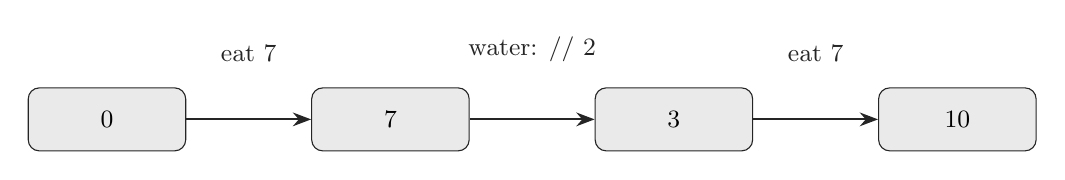
\begin{tikzpicture}[>=Stealth,every node/.style={font=\small},box/.style={draw=teal,rounded corners,minimum width=20mm,minimum height=8mm,fill=wash},arr/.style={->,thick,teal}]\node[box] (p0) at (0.0,0) {0};\node[box] (p1) at (3.6,0) {7};\node[box] (p2) at (7.2,0) {3};\node[box] (p3) at (10.8,0) {10};\draw[arr] (p0)--node[above=6mm]{eat 7}(p1);\draw[arr] (p1)--node[above=6mm]{water: // 2}(p2);\draw[arr] (p2)--node[above=6mm]{eat 7}(p3);\end{tikzpicture}\end{center}\end{minipage}
\par\bigskip\begin{minipage}{\textwidth}\textbf{L4-05 / First, all fullness values before water}\par\par\medskip \begingroup\footnotesize\setlength{\tabcolsep}{4pt}\renewcommand{\arraystretch}{1.35}\begin{tabularx}{\linewidth}{>{\raggedright\arraybackslash}l>{\raggedright\arraybackslash}X>{\raggedright\arraybackslash}X>{\raggedright\arraybackslash}X>{\raggedright\arraybackslash}X>{\raggedright\arraybackslash}X>{\raggedright\arraybackslash}X>{\raggedright\arraybackslash}X>{\raggedright\arraybackslash}X>{\raggedright\arraybackslash}X>{\raggedright\arraybackslash}X>{\raggedright\arraybackslash}X}\toprule\textbf{Fullness f} & \textbf{0} & \textbf{1} & \textbf{2} & \textbf{3} & \textbf{4} & \textbf{5} & \textbf{6} & \textbf{7} & \textbf{8} & \textbf{9} & \textbf{10}\\\midrule
dry[f] & Y & - & - & - & Y & - & - & Y & Y & - & -\\
\bottomrule\end{tabularx}\endgroup\par\medskip \end{minipage}
\par\bigskip\begin{minipage}{\textwidth}\textbf{L4-06 / Then, drink from every dry state}\par\begin{center}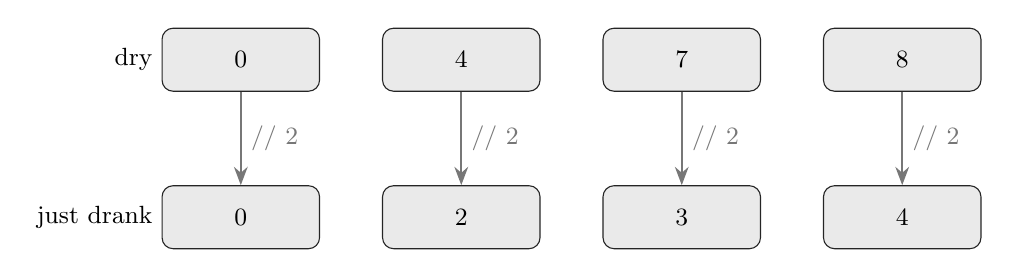
\begin{tikzpicture}[>=Stealth,every node/.style={font=\small},box/.style={draw=teal,rounded corners,minimum width=20mm,minimum height=8mm,fill=wash},arr/.style={->,thick,teal}]\node[anchor=east] at (-1,0) {dry};\node[anchor=east] at (-1,-2) {just drank};\node[box] (a0) at (0.0,0) {0};\node[box] (b0) at (0.0,-2) {0};\draw[arr,orange] (a0)--node[right]{// 2}(b0);\node[box] (a1) at (2.8,0) {4};\node[box] (b1) at (2.8,-2) {2};\draw[arr,orange] (a1)--node[right]{// 2}(b1);\node[box] (a2) at (5.6,0) {7};\node[box] (b2) at (5.6,-2) {3};\draw[arr,orange] (a2)--node[right]{// 2}(b2);\node[box] (a3) at (8.399999999999999,0) {8};\node[box] (b3) at (8.399999999999999,-2) {4};\draw[arr,orange] (a3)--node[right]{// 2}(b3);\end{tikzpicture}\end{center}\end{minipage}
\par\bigskip\begin{minipage}{\textwidth}\textbf{L4-07 / Finally, eat after water}\par\par\medskip \begingroup\footnotesize\setlength{\tabcolsep}{4pt}\renewcommand{\arraystretch}{1.35}\begin{tabularx}{\linewidth}{>{\raggedright\arraybackslash}l>{\raggedright\arraybackslash}X>{\raggedright\arraybackslash}X>{\raggedright\arraybackslash}X>{\raggedright\arraybackslash}X>{\raggedright\arraybackslash}X>{\raggedright\arraybackslash}X>{\raggedright\arraybackslash}X>{\raggedright\arraybackslash}X>{\raggedright\arraybackslash}X>{\raggedright\arraybackslash}X>{\raggedright\arraybackslash}X}\toprule\textbf{Fullness f} & \textbf{0} & \textbf{1} & \textbf{2} & \textbf{3} & \textbf{4} & \textbf{5} & \textbf{6} & \textbf{7} & \textbf{8} & \textbf{9} & \textbf{10}\\\midrule
wet[f] & Y & - & Y & Y & Y & - & Y & Y & Y & Y & Y\\
\bottomrule\end{tabularx}\endgroup\par\medskip \end{minipage}
\par\bigskip\begin{minipage}{\textwidth}\textbf{L4-09 / Your turn: a different feast}\par\par\medskip \begingroup\footnotesize\setlength{\tabcolsep}{4pt}\renewcommand{\arraystretch}{1.35}\begin{tabularx}{\linewidth}{>{\raggedright\arraybackslash}l>{\raggedright\arraybackslash}X>{\raggedright\arraybackslash}X>{\raggedright\arraybackslash}X>{\raggedright\arraybackslash}X>{\raggedright\arraybackslash}X>{\raggedright\arraybackslash}X>{\raggedright\arraybackslash}X>{\raggedright\arraybackslash}X>{\raggedright\arraybackslash}X>{\raggedright\arraybackslash}X}\toprule\textbf{Fullness f} & \textbf{0} & \textbf{1} & \textbf{2} & \textbf{3} & \textbf{4} & \textbf{5} & \textbf{6} & \textbf{7} & \textbf{8} & \textbf{9}\\\midrule
dry[f] & Y & - & - & - & Y & - & Y & - & Y & -\\
just drank & Y & - & Y & Y & Y & - & - & - & - & -\\
wet[f] & Y & - & Y & Y & Y & - & Y & Y & Y & Y\\
\bottomrule\end{tabularx}\endgroup\par\medskip \end{minipage}
\topicflow{CODE ANSWERS}{Complete code}
Every function used in class, in question order. Line numbers are the same as in the tutor book.\par\medskip
\Needspace{25\baselineskip}
{\color{teal}\textbf{L4-04}}\quad\textbf{\texttt{feast\_cached}}\label{L4-code-feast_cached}\par
\begin{lstlisting}[style=numbered]
from functools import lru_cache

def feast_cached(limit, a, b):
    @lru_cache(None)
    def best(fullness, used_water):
        answer = fullness
        for fruit in (a, b):
            if fullness + fruit <= limit:
                answer = max(answer, best(fullness + fruit, used_water))
        if not used_water:
            answer = max(answer, best(fullness // 2, True))
        return answer
    return best(0, False)
\end{lstlisting}
\textbf{Recursion depth.} Python stops recursion at about 1,000 nested calls by default, so this recursive version is for small inputs and the small and edge test files only. Use the iterative version for the medium and large files.


\begin{lstlisting}
print(feast_cached(10, 4, 7))
\end{lstlisting}
\textbf{Expected output:} 10
\par\bigskip
\Needspace{29\baselineskip}
{\color{teal}\textbf{L4-08}}\quad\textbf{\texttt{feast\_table}}\label{L4-code-feast_table}\par
\begin{lstlisting}[style=numbered]
def feast_table(limit, a, b):
    dry = bytearray(limit + 1)
    wet = bytearray(limit + 1)
    dry[0] = 1
    for fullness in range(limit + 1):
        if dry[fullness]:
            for fruit in (a, b):
                if fullness + fruit <= limit:
                    dry[fullness + fruit] = 1
    for fullness in range(limit + 1):
        if dry[fullness]:
            wet[fullness // 2] = 1
    for fullness in range(limit + 1):
        if wet[fullness]:
            for fruit in (a, b):
                if fullness + fruit <= limit:
                    wet[fullness + fruit] = 1
    for fullness in range(limit, -1, -1):
        if dry[fullness] or wet[fullness]:
            return fullness
\end{lstlisting}

\begin{lstlisting}
print(feast_table(10, 4, 7))
\end{lstlisting}
\textbf{Expected output:} 10
\par\bigskip
\topicflow{EXERCISE CHECKS}{Expected notebook results}
\Needspace{8\baselineskip}\textbf{L4-09 / feast\_table}\par
Use the complete \texttt{feast\_table} solution on page~\pageref{L4-code-feast_table}. The function name and parameters are the same in the notebook.

\begin{lstlisting}
feast_table(9, 4, 6)   # expected: 9
feast_table(10, 4, 7)  # expected: 10
\end{lstlisting}
\Needspace{8\baselineskip}\textbf{L4-10 / feast\_table}\par
Use the complete \texttt{feast\_table} solution on page~\pageref{L4-code-feast_table}. The function name and parameters are the same in the notebook.

\begin{lstlisting}
feast_table(1, 1, 1)  # expected: 1
feast_table(8, 4, 6)  # expected: 8
feast_table(5, 4, 4)  # expected: 4
\end{lstlisting}
\clearpage\renewcommand{\lessonnumber}{5}\renewcommand{\lessonheading}{Lesson 5 · Hoof, Paper, Scissors}\phantomsection\label{lesson-5}\pdfbookmark[-1]{Lesson 5: Hoof, Paper, Scissors}{lesson-5-bookmark}
\noindent\makebox[\linewidth][l]{\begin{minipage}{176mm}{\heavy\fontsize{23}{28}\selectfont\raggedright Lesson 5\par}\vspace{2mm}{\heavy\fontsize{19}{24}\selectfont\raggedright Hoof, Paper, Scissors\par}\end{minipage}}\par\vspace{5mm}
\href{https://colab.research.google.com/github/fifteen02/julians-pathfinder/blob/main/Lesson\%205/lesson.ipynb}{\underline{Open this lesson in Google Colab}}\par
\topicflow{BEFORE CLASS}{The lesson route}
\par\noindent\colorbox{wash}{\parbox{\dimexpr\linewidth-2\fboxsep\relax}{\vspace{3pt}{\color{quiet}\heavy\fontsize{8.5}{10}\selectfont MAIN IDEA: SAY THIS AT THE START}\par\smallskip{\heavy\fontsize{15}{18}\selectfont Choose when to switch.}\par\smallskip Keep the round, the switches used and the current gesture; at every round, compare staying with switching.\par\medskip\textbf{By the end of the lesson you will be able to}\begin{itemize}\item record the round, switches used and ending gesture for each score;\item explain why at most K switches is not the same as exactly K switches;\item fill each round from the previous round by comparing stay and switch.\end{itemize}\vspace{3pt}}}\par

The target is understanding, not finishing every page. Use the question IDs to move between slides, worksheet and notebook.

\begingroup\small\setlength{\tabcolsep}{4pt}\renewcommand{\arraystretch}{1.35}\begin{tabularx}{\linewidth}{>{\raggedright\arraybackslash}p{18mm}>{\raggedright\arraybackslash}X>{\raggedright\arraybackslash}p{38mm}}\toprule\textbf{Minutes} & \textbf{Activity} & \textbf{Question IDs}\\\midrule
0-15 & Game rules and no-switch baseline & L5-01 to L5-02\\
15-30 & Find a one-switch strategy & L5-03\\
30-45 & State information and recursive search & L5-04 to L5-05\\
45-60 & Exact usage and impossible states & L5-06\\
60-65 & Break & \\
65-85 & Trace stay and switch candidates & L5-07 to L5-08\\
85-100 & Rolling-table implementation & L5-09\\
100-115 & Student tests and strategy explanation & L5-10 to L5-11\\
115-120 & Exit: explain the three state parts & L5-12\\
\bottomrule\end{tabularx}\endgroup

\labeltext{Pacing and preparation}
Ask students to predict before running code. Allow a quiet individual attempt before asking for a volunteer. If an answer is wrong, trace the first state where it differs. Keep the final ten minutes for explanation and questions. Move an unfinished implementation to the next session rather than shortening the reasoning.

Students need Python functions, lists, loops, indexing, comparisons and basic arithmetic. Introduce new syntax beside the program that uses it. Use small inputs for uncached recursion; the notebook never starts an enormous recursive run. Python stops recursion at about 1,000 nested calls by default, so every recursive version in this lesson, cached or not, is for small inputs and the small and edge test files only. The medium and large files are for the iterative versions.

Open lesson.ipynb in Jupyter or upload it to Google Colab, choose a Python 3 runtime, and run the setup cell first. Shift+Enter runs a cell. Restart and run from the top if names or data become stale. The notebook needs only Python standard-library features and no local files.
\topic{KEEP BESIDE YOUR WORK}{The route and the rules}
\textbf{Our route}\par Count wins when one gesture is kept throughout. Then place one change by hand. To solve longer games, record the round, switches used and ending gesture. Compare keeping that gesture with changing it, and fill a fresh table for each round.\par\medskip
\textbf{Game rules}\par John's entire sequence is known in advance. Bessie chooses H (hoof), P (paper) or S (scissors) for each round. H beats S, S beats P, and P beats H. A win scores 1; a draw or loss scores 0. Maximise Bessie's total wins.\par\medskip
\textbf{Switch rules}\par The first gesture is free. A switch is a change of gesture between two consecutive rounds. The budget, called K in the judge's statement and budget in the code, allows at most that many changes, not exactly that many. For example, H, H, P uses one switch. Number rounds from 0, so round 2 is the third round.\par\medskip
\textbf{Names used in the questions}\par \texttt{used} is the number of switches already used (written \texttt{used} in the code too). \texttt{g} is the current gesture. A score cell stores the most wins among strategies with that exact used and g after the specified round. Two different strategies may contribute to the same cell; keep the better score.\par\medskip
\textbf{Reading the tables}\par The columns headed H, P and S identify Bessie's ending gesture, not John's move. Write a dash for a state that is impossible. A score of 0 instead means a legal strategy exists but has no wins. L5-06 connects the dash to the program's negative-infinity value.\par\medskip
\topicflow{IN CLASS}{Questions, answers and prompts}
\markboth{Plan gestures and count switches}{}{\color{quiet}\heavy\fontsize{10}{13}\selectfont PLAN GESTURES AND COUNT SWITCHES}\par\medskip
\noindent\begin{minipage}{\textwidth}
{\color{teal}\textbf{L5-01}}\quad \textbf{Which gesture wins?}\par\smallskip
\textbf{Ask.} H means hoof, P paper and S scissors. H beats S, S beats P, and P beats H. A win scores 1; a draw or loss scores 0. John plays H, H, S, S, P. Fill Bessie's wins in each round when she keeps H throughout, then when she keeps P or S.\par\smallskip
\textbf{Answer.} Keeping H wins twice, against the two S rounds. Keeping P wins twice, against the two H rounds. Keeping S wins once, against P. Draws and losses each contribute zero wins.\par\smallskip
\textbf{Prompt if stuck.} For each fixed gesture, mark exactly the rounds it beats.\par\smallskip
\textbf{Watch for.} The gesture that beats H is P, not S.
\end{minipage}\par\medskip{\color{lightink}\hrule height .4pt}\medskip

\noindent\begin{minipage}{\textwidth}
{\color{teal}\textbf{L5-02}}\quad \textbf{Zero switches is already a useful case}\par\smallskip
\textbf{Ask.} With no switches allowed, how would you solve the whole game? What answer do you get for H, H, S, S, P?\par\smallskip
\textbf{Answer.} Count the wins for each fixed gesture and take the largest. The answer is 2. Choosing the first gesture is free, so all three fixed strategies are available.\par\smallskip
\textbf{Prompt if stuck.} Choose a gesture once, then score it against every round.\par\smallskip
\textbf{Watch for.} Charging a switch for the first gesture incorrectly excludes all zero-switch strategies.
\end{minipage}\par\medskip{\color{lightink}\hrule height .4pt}\medskip

\noindent\begin{minipage}{\textwidth}
{\color{teal}\textbf{L5-03}}\quad \textbf{One well-placed switch}\par\smallskip
\textbf{Ask.} John plays H, H, S, S, P. Bessie may choose her first gesture freely and change it at most once between rounds. Find a strategy with four wins. Number rounds from 0 and identify the gap where she changes. Can one change produce five wins?\par\smallskip
\textbf{Answer.} Play P, P, H, H, H. Switch once before round 2 and win four rounds. Winning all five would require P, P, H, H, S, which changes twice. Thus 4 is optimal.\par\smallskip
\textbf{Prompt if stuck.} Group John's identical consecutive gestures.\par\smallskip
\textbf{Watch for.} A final loss can be part of an optimal strategy when switches are limited.
\end{minipage}\par\medskip{\color{lightink}\hrule height .4pt}\medskip

\noindent\begin{minipage}{\textwidth}
{\color{teal}\textbf{L5-04}}\quad \textbf{What must the state remember?}\par\smallskip
\textbf{Ask.} Two strategies have processed the same rounds and used one switch, but one ends with H and the other with P. Can their best win counts be merged into one number?\par\smallskip
\textbf{Answer.} No. Their current gestures differ, so the next gesture may require a switch in one history but not the other. Record the processed round, switches used and current gesture.\par\smallskip
\textbf{Prompt if stuck.} Consider whether choosing H next consumes a switch in each history.\par\smallskip
\textbf{Watch for.} A history with more wins can still be unsuitable if it has a different gesture or spent budget.
\end{minipage}\par\medskip{\color{lightink}\hrule height .4pt}\medskip

\Needspace{14\baselineskip}\markboth{Store scores and compare continuations}{}{\color{quiet}\heavy\fontsize{10}{13}\selectfont STORE SCORES AND COMPARE CONTINUATIONS}\par\medskip
\noindent\begin{minipage}{\textwidth}
{\color{teal}\textbf{L5-05}}\quad \textbf{Recursive choices with a budget}\par\smallskip
\textbf{Ask.} Write hps\_cached(john, budget) using recursion. Its helper knows the next round, switches left and previous gesture. How do you handle the first round without charging a switch?\par\smallskip
\par\smallskip{\small\textbf{Students start with:}}\par\smallskip\noindent\colorbox{codepaper}{\parbox{\dimexpr\linewidth-2\fboxsep\relax}{\small\ttfamily\raggedright def hps\_cached(john, budget):\\\hspace*{2.4em}def best(i, left, previous):\\\hspace*{4.8em}return None  \# Your helper goes here.\\\hspace*{2.4em}return best(0, budget, '')}}\par
{\small\textbf{What each function returns.}\par hps\_cached(john, budget): the most rounds Bessie can win within the switch budget.\par best(i, left, previous): the most further wins from round i, with left switches available and previous as the last gesture.\par }
{\small\textbf{Hints to give, one at a time.}}\begin{itemize}\item What does best return when no rounds remain?\item When does choosing a gesture cost a switch, and when is it free?\item Which choices are not allowed with the switches left?\end{itemize}
\textbf{Answer.} Try each gesture. Charge one switch only if a previous gesture exists and the new one differs. Reject choices that exceed the remaining budget. Add this round's win to the best continuation.\par\smallskip
\textbf{Prompt if stuck.} The first gesture has no earlier gesture to differ from.\par\smallskip
\textbf{Watch for.} Subtracting a switch on the first round breaks budget-zero cases.\par\smallskip Full code: \texttt{hps\_cached} (page~\pageref{L5-code-hps_cached}).
\end{minipage}\par\medskip{\color{lightink}\hrule height .4pt}\medskip

\noindent\begin{minipage}{\textwidth}
{\color{teal}\textbf{L5-06}}\quad \textbf{Exactly used versus at most allowed}\par\smallskip
\textbf{Ask.} John plays H in round 0. Fill Bessie's scores for each ending gesture H, P and S with exactly zero switches used. Can exactly one switch have been used after just this round? Write a dash for impossible states and explain why a score of 0 would mean something different.\par\smallskip
\textbf{Answer.} For ending gestures H, P, S, the zero-switch scores are [0, 1, 0]. Exactly one switch is impossible after one round. Mark impossible states with negative infinity, not zero.\par\smallskip
\textbf{Prompt if stuck.} A switch happens between rounds, not before the first round.\par\smallskip
\textbf{Watch for.} Exact-state semantics and at-most-state semantics require different initialisation rules.
\end{minipage}\par\medskip{\color{lightink}\hrule height .4pt}\medskip

\noindent\begin{minipage}{\textwidth}
{\color{teal}\textbf{L5-07}}\quad \textbf{Stay or switch before this round}\par\smallskip
\textbf{Ask.} After John plays H,H, scores for ending H,P,S are [0,2,0] with no switches and [1,1,1] with exactly one. John now plays S. For an ending H with exactly one switch, compare staying with H against changing from P or S. Then fill both new score rows.\par\smallskip
\textbf{Answer.} Stay with H after one earlier switch: 1 + 1 = 2. Switch now from P: 2 + 1 = 3; from S: 0 + 1 = 1. Each candidate adds this round's win once. Keep 3. The complete rows are [1,2,0] for zero switches and [3,1,2] for exactly one.\par\smallskip
\textbf{Prompt if stuck.} The old gesture that won both H rounds was P.\par\smallskip
\textbf{Watch for.} Reading the same switch-count row for a change would allow switches for free.
\end{minipage}\par\medskip{\color{lightink}\hrule height .4pt}\medskip

\noindent\begin{minipage}{\textwidth}
{\color{teal}\textbf{L5-08}}\quad \textbf{Trace all five rounds}\par\smallskip
\textbf{Ask.} Trace John's rounds H,H,S,S,P. In each table column, 0 or 1 is the exact number of switches used; H, P or S is Bessie's ending gesture. Fill every row from the row immediately above it. A dash means impossible. Which final entry gives the best score with at most one switch?\par\smallskip
\textbf{Answer.} After all five rounds, zero-switch scores are [2,2,1] and one-switch scores are [4,2,3]. The largest score across both rows is 4, ending with H after one switch.\par\smallskip
\textbf{Prompt if stuck.} At each round, add a win only to the gesture that beats John's move.\par\smallskip
\textbf{Watch for.} The final answer may use fewer switches than the budget.
\end{minipage}\par\medskip{\color{lightink}\hrule height .4pt}\medskip

\noindent\begin{minipage}{\textwidth}
{\color{teal}\textbf{L5-09}}\quad \textbf{Keep just the previous round}\par\smallskip
\textbf{Ask.} Write hps\_table(john, budget) using a loop over rounds. Here used counts switches already used and g is the ending gesture. before[used][g] stores the best score after the previous round; now[used][g] includes the current round. Compare staying and switching. Why must now be fresh? Return the best score using at most budget switches (K in the original statement).\par\smallskip
\par\smallskip{\small\textbf{Students start with:}}\par\smallskip\noindent\colorbox{codepaper}{\parbox{\dimexpr\linewidth-2\fboxsep\relax}{\small\ttfamily\raggedright def hps\_table(john, budget):\\\hspace*{2.4em}return None  \# Replace with your answer.}}\par
{\small\textbf{What each function returns.}\par hps\_table(john, budget): the most rounds Bessie can win within the switch budget.\par }
{\small\textbf{Hints to give, one at a time.}}\begin{itemize}\item What are the scores after round 0, and which states are impossible then?\item For a new cell, which cells of before lead to it by staying, and which by switching?\item What should an impossible state hold so that max ignores it?\end{itemize}
\textbf{Answer.} before holds completed scores for the previous round; now holds scores for the current round. Keep the old table unchanged while all new cells are calculated, so a round cannot be counted twice. For at most K switches, return the maximum over every ending gesture and every usage row from 0 to K.\par\smallskip
\textbf{Prompt if stuck.} Every candidate must come from before, never from a partially filled now.\par\smallskip
\textbf{Watch for.} Updating one table in place can reuse the current round more than once.\par\smallskip Full code: \texttt{hps\_table} (page~\pageref{L5-code-hps_table}).
\end{minipage}\par\medskip{\color{lightink}\hrule height .4pt}\medskip

\Needspace{14\baselineskip}\markboth{Test the budget and explain the state}{}{\color{quiet}\heavy\fontsize{10}{13}\selectfont TEST THE BUDGET AND EXPLAIN THE STATE}\par\medskip
\noindent\begin{minipage}{\textwidth}
{\color{teal}\textbf{L5-10}}\quad \textbf{Your turn: three different budgets}\par\smallskip
\textbf{Ask.} Test your hps\_table(john, budget) from L5-09. For John = H,P,S, predict the best win count with budgets 0, 1 and 2. Give one strategy for each budget, then run your function.\par\smallskip
\textbf{Answer.} Budget 0: 1 win, for example P,P,P. Budget 1: 2 wins, for example P,S,S. Budget 2: 3 wins with P,S,H. The first gesture is free in every case.\par\smallskip
\textbf{Prompt if stuck.} Write the uniquely winning gesture under each opponent move.\par\smallskip
\textbf{Watch for.} An available switch need not be spent; it is a maximum allowance.
\end{minipage}\par\medskip{\color{lightink}\hrule height .4pt}\medskip

\noindent\begin{minipage}{\textwidth}
{\color{teal}\textbf{L5-11}}\quad \textbf{More switches need not help}\par\smallskip
\textbf{Ask.} Test your hps\_table(john, budget) from L5-09 on John = H,H,H with budgets 0 and 2, and on one round against S with budget 0. Predict each answer before running it. What should happen when the budget exceeds the useful number of changes?\par\smallskip
\textbf{Answer.} For H,H,H, both budgets give 3 wins by keeping P. For one S round the answer is 1 by choosing H, with no switch needed. Extra budget never forces extra changes.\par\smallskip
\textbf{Prompt if stuck.} The strategy that won before remains legal when more switches are allowed.\par\smallskip
\textbf{Watch for.} Exactly K switches is not the same requirement as at most K switches.
\end{minipage}\par\medskip{\color{lightink}\hrule height .4pt}\medskip

\noindent\begin{minipage}{\textwidth}
{\color{teal}\textbf{L5-12}}\quad \textbf{The state is the explanation}\par\smallskip
\textbf{Ask.} Choose a cell from the five-round score table and explain its round, exact switch count, ending gesture and stored score. Why can we forget the earlier gesture sequence once these facts and its best score are known? Compare this with Tower or Array Description.\par\smallskip
\textbf{Answer.} After H,H,S, the cell for exactly one switch and ending H stores 3: P,P,H wins every round. A worse strategy at that same round, usage and gesture cannot improve future choices: it has the same remaining moves but fewer wins. Tower similarly keeps position and next player; Array Description keeps position and previous value.\par\smallskip
\textbf{Prompt if stuck.} Include round, switches used, ending gesture and the unit of the stored value.\par\smallskip
\textbf{Watch for.} A three-dimensional table is a representation, not an explanation on its own.
\end{minipage}\par\medskip{\color{lightink}\hrule height .4pt}\medskip

\topicflow{TRACE ANSWERS}{Completed diagrams and tables}
\par\bigskip\begin{minipage}{\textwidth}\textbf{L5-01 / Which gesture wins?}\par\par\medskip \begingroup\small\setlength{\tabcolsep}{4pt}\renewcommand{\arraystretch}{1.35}\begin{tabularx}{\linewidth}{>{\raggedright\arraybackslash}X>{\raggedright\arraybackslash}X>{\raggedright\arraybackslash}X>{\raggedright\arraybackslash}X>{\raggedright\arraybackslash}X>{\raggedright\arraybackslash}X}\toprule\textbf{Round} & \textbf{0} & \textbf{1} & \textbf{2} & \textbf{3} & \textbf{4}\\\midrule
John & H & H & S & S & P\\
Keep H & 0 & 0 & 1 & 1 & 0\\
Keep P & 1 & 1 & 0 & 0 & 0\\
Keep S & 0 & 0 & 0 & 0 & 1\\
\bottomrule\end{tabularx}\endgroup\par\medskip \end{minipage}
\par\bigskip\begin{minipage}{\textwidth}\textbf{L5-03 / One well-placed switch}\par\par\medskip \begingroup\small\setlength{\tabcolsep}{4pt}\renewcommand{\arraystretch}{1.35}\begin{tabularx}{\linewidth}{>{\raggedright\arraybackslash}X>{\raggedright\arraybackslash}X>{\raggedright\arraybackslash}X>{\raggedright\arraybackslash}X>{\raggedright\arraybackslash}X>{\raggedright\arraybackslash}X}\toprule\textbf{Round} & \textbf{0} & \textbf{1} & \textbf{2} & \textbf{3} & \textbf{4}\\\midrule
John & H & H & S & S & P\\
Bessie & P & P & H & H & H\\
Wins & 1 & 1 & 1 & 1 & 0\\
\bottomrule\end{tabularx}\endgroup\par\medskip \end{minipage}
\par\bigskip\begin{minipage}{\textwidth}\textbf{L5-06 / Exactly used versus at most allowed}\par\par\medskip \begingroup\small\setlength{\tabcolsep}{4pt}\renewcommand{\arraystretch}{1.35}\begin{tabularx}{\linewidth}{>{\raggedright\arraybackslash}X>{\raggedright\arraybackslash}X>{\raggedright\arraybackslash}X>{\raggedright\arraybackslash}X}\toprule\textbf{Switches used} & \textbf{End H} & \textbf{End P} & \textbf{End S}\\\midrule
0 & 0 & 1 & 0\\
1 & impossible & impossible & impossible\\
\bottomrule\end{tabularx}\endgroup\par\medskip \end{minipage}
\par\bigskip\begin{minipage}{\textwidth}\textbf{L5-07 / Stay or switch before this round}\par\par\medskip \begingroup\small\setlength{\tabcolsep}{4pt}\renewcommand{\arraystretch}{1.35}\begin{tabularx}{\linewidth}{>{\raggedright\arraybackslash}X>{\raggedright\arraybackslash}X>{\raggedright\arraybackslash}X>{\raggedright\arraybackslash}X}\toprule\textbf{After H,H,S} & \textbf{End H} & \textbf{End P} & \textbf{End S}\\\midrule
0 switches & 1 & 2 & 0\\
1 switch & 3 & 1 & 2\\
\bottomrule\end{tabularx}\endgroup\par\medskip \end{minipage}
\par\bigskip\begin{minipage}{\textwidth}\textbf{L5-08 / Trace all five rounds}\par\par\medskip \begingroup\small\setlength{\tabcolsep}{4pt}\renewcommand{\arraystretch}{1.35}\begin{tabularx}{\linewidth}{>{\raggedright\arraybackslash}l>{\raggedright\arraybackslash}X>{\raggedright\arraybackslash}X>{\raggedright\arraybackslash}X>{\raggedright\arraybackslash}X>{\raggedright\arraybackslash}X>{\raggedright\arraybackslash}X}\toprule\textbf{John prefix} & \textbf{0: H} & \textbf{0: P} & \textbf{0: S} & \textbf{1: H} & \textbf{1: P} & \textbf{1: S}\\\midrule
H & 0 & 1 & 0 & - & - & -\\
HH & 0 & 2 & 0 & 1 & 1 & 1\\
HHS & 1 & 2 & 0 & 3 & 1 & 2\\
HHSS & 2 & 2 & 0 & 4 & 1 & 2\\
HHSSP & 2 & 2 & 1 & 4 & 2 & 3\\
\bottomrule\end{tabularx}\endgroup\par\medskip \end{minipage}
\par\bigskip\begin{minipage}{\textwidth}\textbf{L5-12 / The state is the explanation}\par\par\medskip \begingroup\small\setlength{\tabcolsep}{4pt}\renewcommand{\arraystretch}{1.35}\begin{tabularx}{\linewidth}{>{\raggedright\arraybackslash}X>{\raggedright\arraybackslash}X>{\raggedright\arraybackslash}X>{\raggedright\arraybackslash}X}\toprule\textbf{John prefix} & \textbf{Switches used} & \textbf{Ending gesture} & \textbf{Stored score}\\\midrule
HHS & 1 & H & 3\\
\bottomrule\end{tabularx}\endgroup\par\medskip \end{minipage}
\topicflow{CODE ANSWERS}{Complete code}
Every function used in class, in question order. Line numbers are the same as in the tutor book.\par\medskip
\Needspace{29\baselineskip}
{\color{teal}\textbf{L5-05}}\quad\textbf{\texttt{hps\_cached}}\label{L5-code-hps_cached}\par
\begin{lstlisting}[style=numbered]
from functools import lru_cache

BEATS = {'H': 'S', 'P': 'H', 'S': 'P'}

def hps_cached(john, budget):
    @lru_cache(None)
    def best(i, left, previous):
        if i == len(john):
            return 0
        answer = 0
        for gesture in 'HPS':
            change = int(previous != '' and gesture != previous)
            if change <= left:
                win = int(BEATS[gesture] == john[i])
                answer = max(answer, win + best(i + 1, left - change, gesture))
        return answer
    return best(0, budget, '')
\end{lstlisting}
\textbf{Recursion depth.} Python stops recursion at about 1,000 nested calls by default, so this recursive version is for small inputs and the small and edge test files only. Use the iterative version for the medium and large files.


\begin{lstlisting}
print(hps_cached('HHSSP', 1))
\end{lstlisting}
\textbf{Expected output:} 4
\par\bigskip
\Needspace{31\baselineskip}
{\color{teal}\textbf{L5-09}}\quad\textbf{\texttt{hps\_table}}\label{L5-code-hps_table}\par
\begin{lstlisting}[style=numbered]
BEATS = {'H': 'S', 'P': 'H', 'S': 'P'}

def hps_table(john, budget):
    if not john:
        return 0
    gestures = 'HPS'
    impossible = -float('inf')
    before = [[impossible] * 3 for _ in range(budget + 1)]
    for g, gesture in enumerate(gestures):
        before[0][g] = int(BEATS[gesture] == john[0])
    for opponent in john[1:]:
        now = [[impossible] * 3 for _ in range(budget + 1)]
        for used in range(budget + 1):
            for g, gesture in enumerate(gestures):
                best_before = before[used][g]
                if used > 0:
                    for old in range(3):
                        if old != g:
                            best_before = max(best_before, before[used - 1][old])
                now[used][g] = best_before + int(BEATS[gesture] == opponent)
        before = now
    return int(max(max(row) for row in before))
\end{lstlisting}

\begin{lstlisting}
print(hps_table('HHSSP', 1))
\end{lstlisting}
\textbf{Expected output:} 4
\par\bigskip
\topicflow{EXERCISE CHECKS}{Expected notebook results}
\Needspace{8\baselineskip}\textbf{L5-10 / hps\_table}\par
Use the complete \texttt{hps\_table} solution on page~\pageref{L5-code-hps_table}. The function name and parameters are the same in the notebook.

\begin{lstlisting}
hps_table('HPS', 0)    # expected: 1
hps_table('HPS', 1)    # expected: 2
hps_table('HPS', 2)    # expected: 3
hps_table('HHSSP', 1)  # expected: 4
\end{lstlisting}
\Needspace{8\baselineskip}\textbf{L5-11 / hps\_table}\par
Use the complete \texttt{hps\_table} solution on page~\pageref{L5-code-hps_table}. The function name and parameters are the same in the notebook.

\begin{lstlisting}
hps_table('HHH', 0)  # expected: 3
hps_table('HHH', 2)  # expected: 3
hps_table('S', 0)    # expected: 1
\end{lstlisting}
\end{document}
